~\label{chap:spp}
\begin{chapterabstract}
This chapter introduces an approach to the simultaneous prediction of object shape 
and pose from stereo image pairs. A novel, data driven approach is taken that utilises 
the representational power of Convolutional Neural Networks with the generative power of 
Gaussian Processes.
\end{chapterabstract}
% TODO: extend this abstract.

\section{Introduction}
~\label{sec:spp_introduction}
In the computer vision literature, there has been much research on the reconstruction of objects
from observed points in a range image, such as those obtained with an RGBD sensor (like 
the Microsoft Kinect). As outlined in Chapter~\ref{chap:probobj}, progress has been made 
on the techniques used, such that globally consistent models of an object of interest can 
easily be obtained.

Though the traditional reconstruction paradigm is suitable for tasks such as 3D data 
collection, it is less applicable in scenarios where full sensor coverage of the object 
of interest is not possible, as outlined in the research problems in Section
~\ref{sec:intro_aims_structure}. When a full view of an object is not available, only a 
partial reconstruction may be built. Data driven, learning based approaches that yield 
reconstructions as predictions from a generative model do not have such a limitation. 
However, for application as a direct replacement for manual reconstruction, pose estimation 
must also be performed.

There has been much progress on learning based methods for both pose estimation and 
shape prediction, as outlined in Section~\ref{sec:lit_review_prediction}. However, much of 
this progress has been on the two problems when decoupled. In this work, an approach is 
proposed to solve the problem of simultaneous shape and pose prediction. The first 
difference in this work to those outlined in Chapters~\ref{chap:moseg} and~\ref{chap:probobj} 
is the use of monocular RGB frames versus RGBD\@. The central reason for the change of input data 
format is that the use of RGBD is prohibitive when considering outdoor environments where lighting 
conditions may prevent RGBD sensors, such as the Microsoft Kinect, from producing a meaningful depth map.

The second major deviation from the contributions of Chapters~\ref{chap:moseg} and~\ref{chap:probobj} 
is the removal of the dependence on temporally consistent input sequences. Rather, in this work 
the proposed system performs shape and pose prediction from an instantaneous, monocular RGB frame, 
requiring no temporal consistency in both the training and prediction phases. As such, there is no 
iterative solving for shape and pose per frame, rather, the process is framed as an instantaneous 
regression task. However, this work makes use of volumetric shape representations, as with the other 
works outlined in Chapters~\ref{chap:moseg} and~\ref{chap:probobj}.

The approach outlined in this chapter makes use of CNN's and GPLVM's to jointly regress shape and pose 
given an RGB frame with an object (or objects) of interest present in the view frustum. The training of 
the model is part supervised (pose) and part semi-supervised (3D shape), requiring a ground truth 6DoF pose and 
a segmentation of the object(s) of interest. The proposed system regresses rotational and translational 
parameters directly from the neural network component, whilst the object shape drawn from a GPLVM prior\@. 
The use of a GPLVM for latent space embeddings of 3D shape allows for a simple way to learn complex 3D 
geometrical features, thus simplifying the learning tasks of the neural network. In the proposed approach, 
the neural network component need only learn a mapping from observation to latent space, rather than from 
observation to full geometry for the shape of interest.

The system is based on the \textit{Faster-RCNN} approach of \textit{Ren et al}~\cite{Ren2015RCNN}, trained 
on a multi-task loss over detection, classification, pose and shape. For training of shape, the loss is evaluated 
in terms of a rendering of the predicted shape under it's associated pose, against a ground truth segmentation. 
As such, the shape component of the model is trained in a weakly-supervised manner, as there is no ground truth 
3D shape. Though such an approach presents a greater challenge than in the case of known ground truth for 3D shape, 
it does widen the applicability of the approach. In many \textit{real world} scenarios it is not possible to obtain 
such ground truth data without first solving the problem of this work.

As outlined previously, the proposed approach differs from that of Chapters~\ref{chap:moseg} and~\ref{chap:probobj} 
in that it is data driven. Rather than predetermined algorithmic procedures being performed at each frame, the 
result of the input frames is derived from a trained model. As outlined in Sections~\ref{sec:intro_spp} and
~\ref{sec:intro_aims_structure}, the research interest is in shape and pose prediction for objects in larger scale, 
\textit{real world} environments. However, due to the difficulty faced with earlier experiments with a fully semi-supervised 
approach, a ground truth 6DoF pose is highly desirabe. As such, the dataset used in this work is the \textit{Virtual KITTI (VKITTI)} 
dataset~\cite{Gaidon2016}, a photo-realistic, synthetic rendering of the \textit{The KITTI Vision Benchmark Suite}~\cite{Geiger2013,Menze2015,Geiger2012}. 
The advantage of using the aformentioned dataset is the balance between being a real world dataset and having a reliable and 
accurate ground truth for pose. The object class of interest in this work is cars.

The remainder of this chapter is structured as follows; Section~\ref{sec:spp_algorithm} introduces the high level 
structure of the proposed model and the structure of it's neural network components. Section~\ref{sec:spp_gplvm} 
introduces and derives the GPLVM that provides a generative model over shape. Following the introduction 
of the GPLVM, Section~\ref{sec:spp_latent_shape_est} outlines the process of extracting a candidate shape for the observed 
object segmentation, from the GPLVM\@. Sections~\ref{sec:spp_pose_estim} and~\ref{sec:spp_rendering} outline the attitude 
representation of pose and shape rendering method used. Though, these are akin to those of Sections
~\ref{subsub:moseg_static_camera_attitude} and~\ref{subsec:moseg_static_rendering} respectively, the rendering stage is 
modified to introduce the property of differentiability. Sections~\ref{sec:spp_loss} and~\ref{sec:spp_backprop} 
outline the loss function of the model and it's gradient for backpropagation, respectively. Sections~\ref{sec:spp_qualitative} 
and~\ref{sec:spp_quantitative} provide qualitative and quantitative results on the aforementioned dataset, respectively. 
Finally, Section~\ref{sec:spp_discussion} provides a summary of the approach taken in this work and the preliminary results 
of it's use.

\section{Algorithmic Overview}
~\label{sec:spp_algorithm}
The proposed model takes as input a monocular RGB frame with the object(s) of interest present within the 
view frustum. From this RGB frame, a ResNet-101~\cite{He2015} extracts feature descriptors which are mapped 
to a number of candidate object detections~\cite{Girshick2014,Girshick2015_2}. For each detection, the extracted 
feature set is used to regress a latent space point for shape, and six \( \mathbb{SE}(3) \) pose parameters, forming 
a Lie Algebra. The generated shape corresponding to the proposed latent space point is drawn from the distribution 
of the Gaussian Process (GP) prior conditioned on the latent space point. The form of the pose is the Lie 
Group mapping of the parameters, as given in Sections~\ref{subsub:moseg_static_camera_attitude} 
and~\ref{subsec:probobj_analytic_alignment_map}. 

The loss function over the regressed shape and pose is quantified by rendering the generated shape 
under the predicted pose and computing a comparitive loss between the rendered region versus the provided semantic 
segmentation region. To maintain continuity, the rendering operation is formulated in a differentiable manner. As there 
is often no ground 3D shape for \textit{real world} data, training is performed in a weakly-supervised manner against a 
segmentation of the object of interest.

\subsection{Model Architecture}
~\label{subsec:spp_network_architecture}
The model of the proposed approach is of an RCNN~\cite{Girshick2014} like architecture, where for a 
given input frame, a backbone network computes a feature map which is then provided to a Region 
Proposal Network (RPN), responsible for providing candidate Regions of Interest (RoI) in the input image. 
A high level depiction of this architecture is given in Figure~\ref{figure:spp_rcnn}.
For the application outlined in this work, a true positive RoI corresponds to an object for which pose and 
shape should be regressed. From end to end, the model contains a ResNet-101~\cite{He2015} backbone, an RPN,
linear layers, batch normalisation layers, non-linear activations, a mapping from Lie algebra to 
Lie group (for pose), a GPLVM followed by an Inverse Discrete Cosine Transform (IDCT), a ray-caster and 
and a loss layer. As previously outlined, the loss consists of supervised and semi-supervised terms.

\begin{figure}[!htbp]
  \centering
  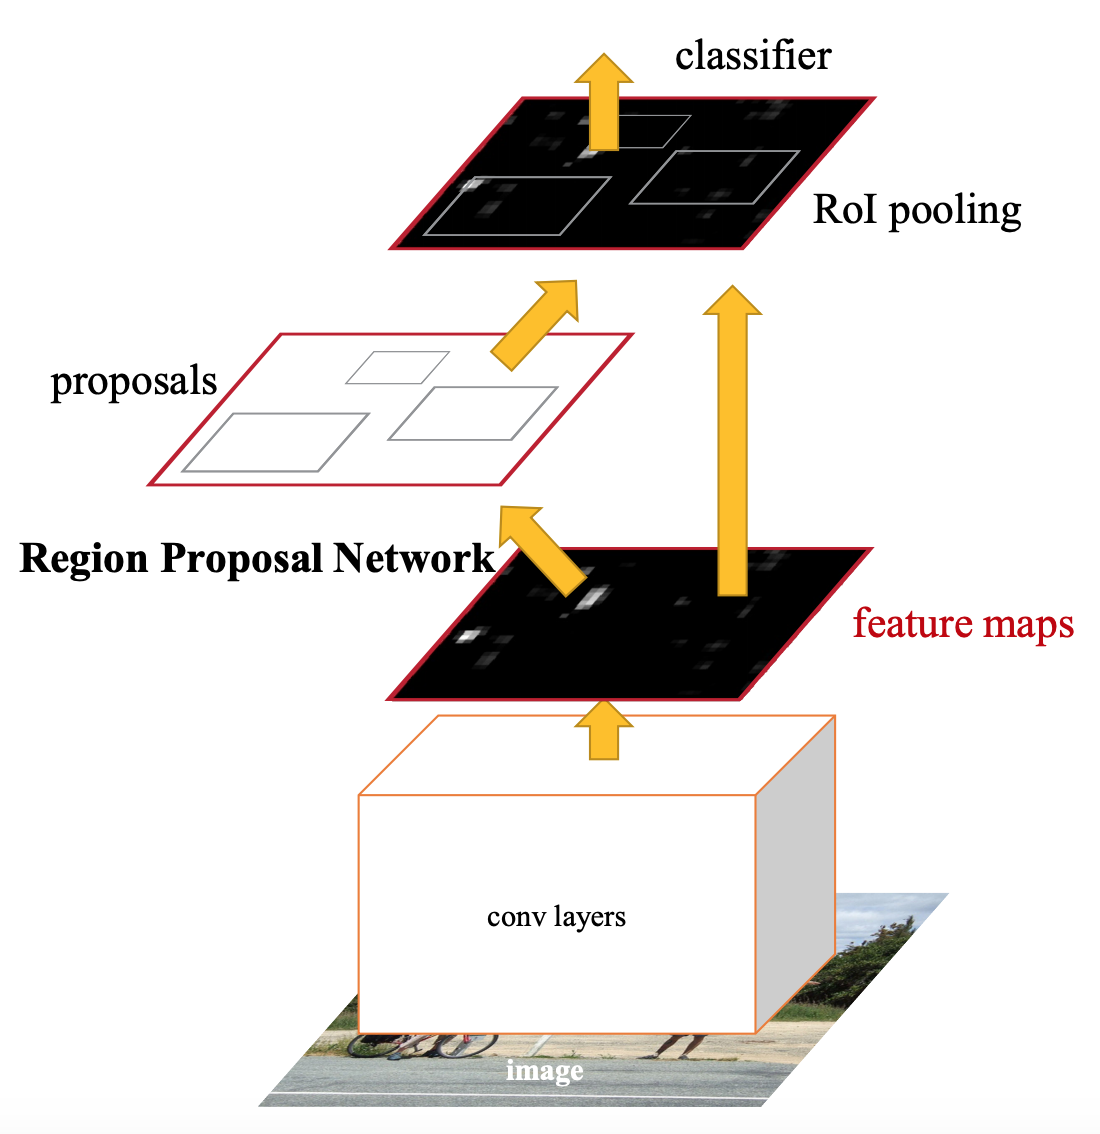
\includegraphics[width=.4\linewidth]{figures/spp/rcnn.png}
  \caption[RCNN Architecture]{Faster R-CNN Architecture.\footnotemark}
~\label{figure:spp_rcnn}
\end{figure}
~\footnotetext{Image copyright: \textit{Ren et al}~\cite{Ren2015RCNN}.}

The purpose of the ResNet-101 and RPN components is to extract, for each region proposal (object proposal), 
feature maps from the input frame that are descriptive of the object of interest in relation to the scene. 
Each proposed feature maps is input into two sub-networks consisting of linear transforms and non-linear activations. 
The purpose of these sub-networks is to regress a latent space point for object shape, and a 6DoF pose parameter vector 
for the object pose.  Following these two sub-networks is the aforementioned GPLVM and Lie algebra mapping. The 
GPLVM generates a posterior mean over shape for a given latent space point, whilst the 
Lie algebra mapping generates an \( \mathbb{SE}(3) \) transform. 

The IDCT decompresses the posterior mean output of the GPLVM to generate a valid SDF\@. Both the 
resultant SDF and \( \mathbb{SE}(3) \) transform are passed to the ray-casting module, which generates 
a rendering for the candidate shape under the predicted pose. Finally, both this rendering and the ground truth 
segmentation mask are passed to the loss layer which computes a similarity metric between the two masks (ground truth and rendered), 
providing a tractible proxy loss for 3D shape. The topology of the proposed model is outlined in Figure~\ref{figure:spp_pipeline}.
\begin{landscape}
  \begin{figure}[!htbp]
    \centering
    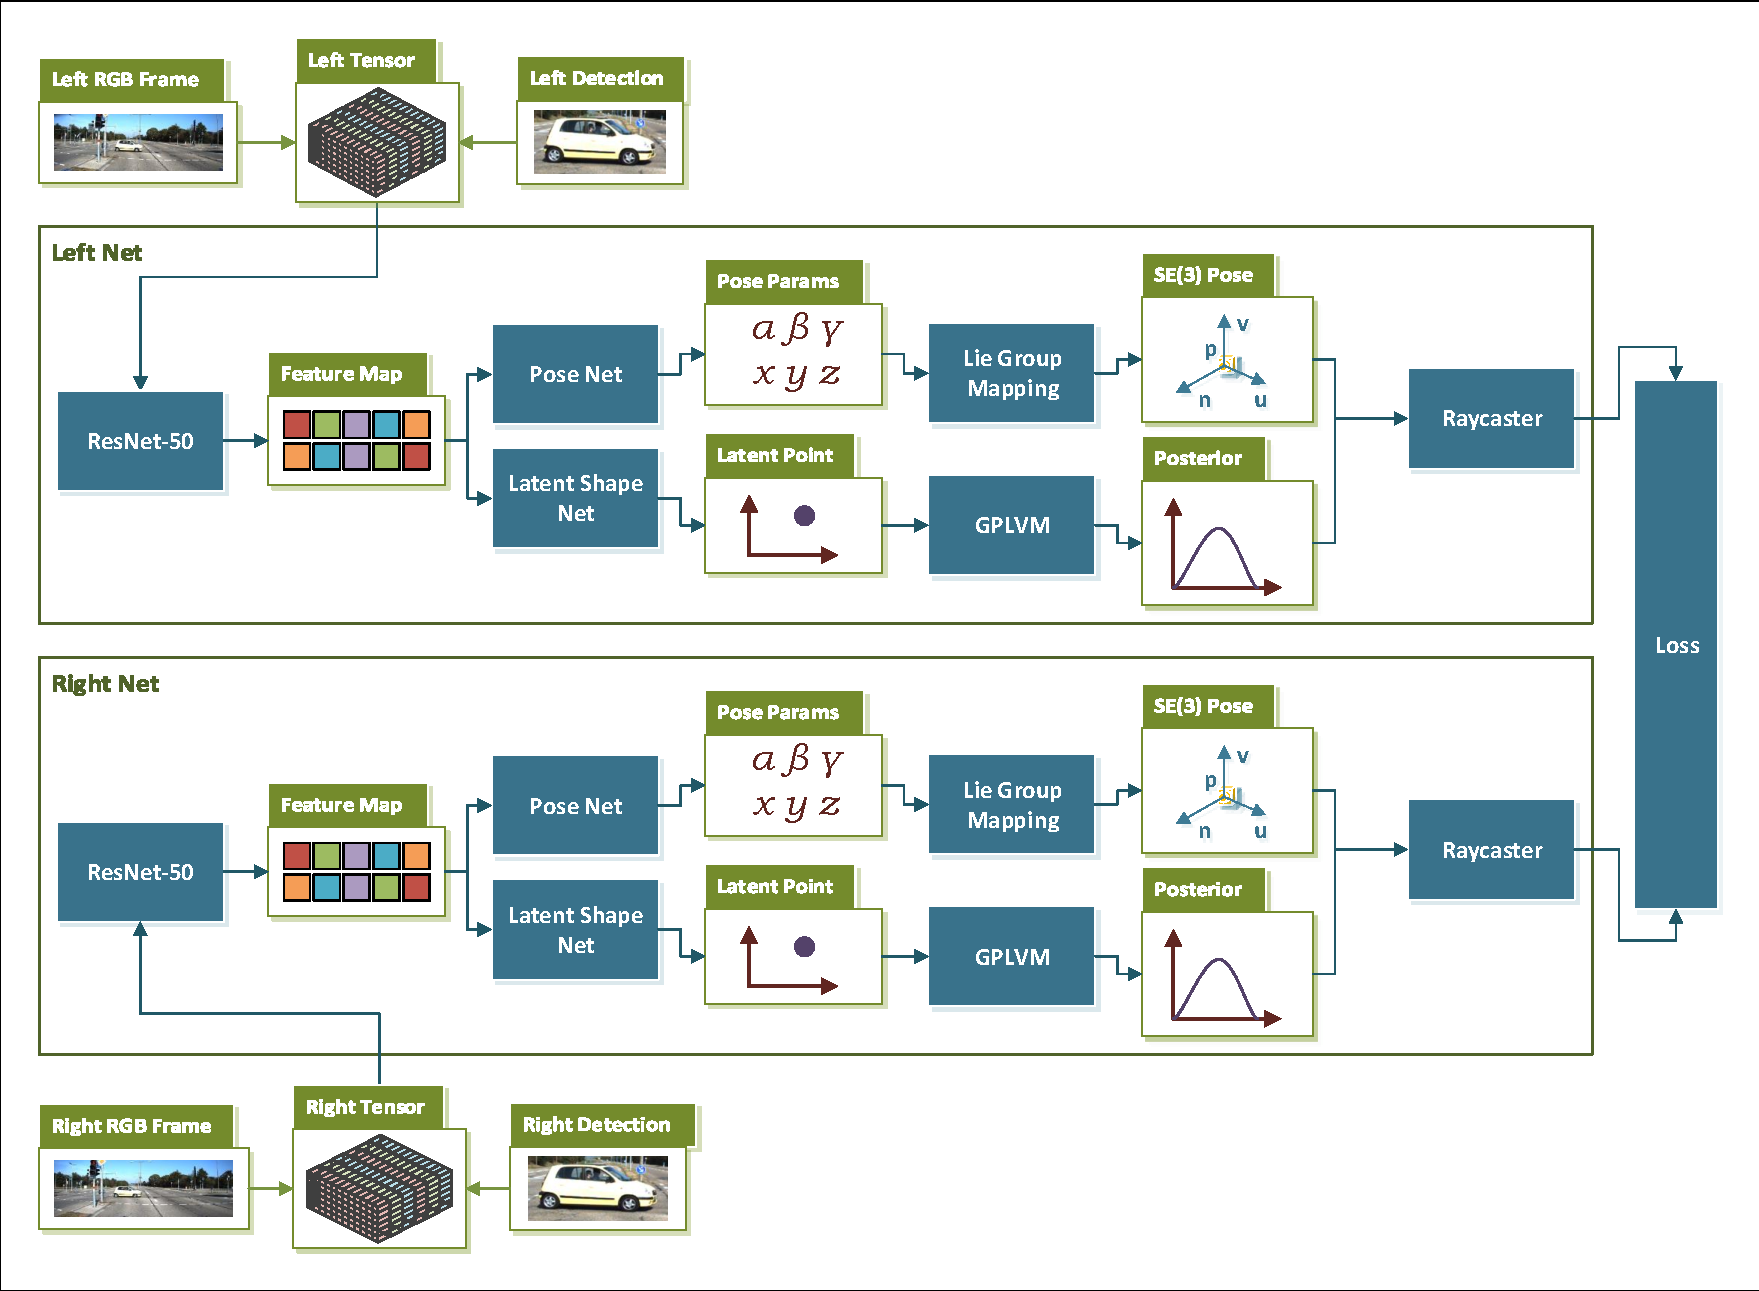
\includegraphics[width=\linewidth]{figures/spp/model.pdf}
    \caption[Shape and Pose Prediction Network]{The proposed shape and pose prediction network. 
    Note that the \textit{ResNet-50}, \textit{Shape Net} and \textit{Latent Net} components have 
    shared parameters.}
~\label{figure:spp_pipeline}
  \end{figure}
\end{landscape}

\subsubsection{Backbone Component}
~\label{subsub:spp_neural_backbone}
The ResNet architecture, introduced by \textit{He at al}~\cite{He2015}, is designed to overcome the 
convergence challenges of very ``deep'' neural network models. The central reformulation in the 
ResNet model is the notion that layers learn \textit{residual functions} with respect to 
their inputs. Instead of a layer learning a mapping \( \mathcal{H}(\bm{x}) \) of it's input \( \bm{x} \), 
it learns a \textit{residual} mapping, as given in Equation~\ref{eqn:resnet}.
\begin{align}
~\label{eqn:resnet}
  \mathcal{F}(\bm{x}) ={}& \mathcal{H}(\bm{x}) - \bm{x}\\
  \mathcal{F}(\bm{x}) + \bm{x} ={}& \mathcal{H}(\bm{x})
\end{align}

The formulation of Equation~\ref{eqn:resnet} is depicted in Figure~\ref{figure:resnet_block}.
\begin{figure}[!htbp]
  \centering
  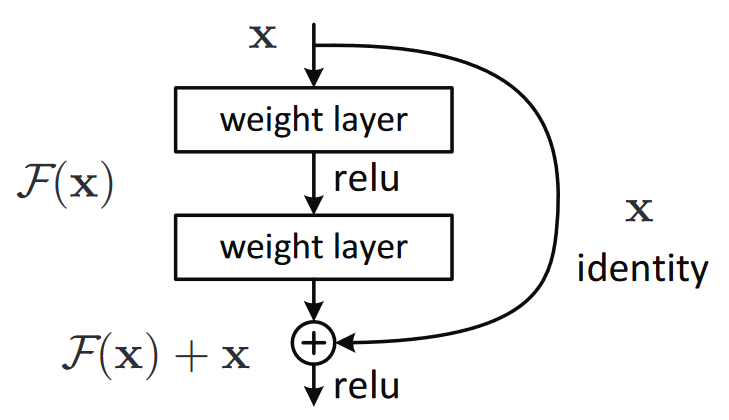
\includegraphics[width=.6\linewidth]{figures/spp/residual_block_he.png}
  \caption[ResNet Block]{The central building block of the ResNet architecture\footnotemark, for some input \( \bm{x} \) and 
  transform \( \mathcal{F} \).}
~\label{figure:resnet_block}
\end{figure}
~\footnotetext{Image copyright: \textit{He et al}~\cite{He2015}.}

\subsubsection{Region Proposal, Classification and Bounding Box Components}
~\label{subsub:spp_neural_rpn}
As outlined in the \textit{Faster-RCNN}~\cite{He2017} literature, the standard 
\textit{R-CNN}~\cite{Girshick2014,Girshick2015_2} architecture contains a region proposal 
network, providing pooled object RoI's in the input image, a classification network and 
a bounding box regression network, as depicted in Figure~\ref{figure:spp_rcnn}.

The standard \textit{R-CNN} components are trained in a supervised manner with ground truth 
bounding boxes and classification labels. In the standard approach, the overall network loss 
is an aggregate of these individual task oriented losses.

\subsubsection{Pose Regression Component}
~\label{subsub:spp_neural_pose}
For each feature map obtained from an RoI object proposal, a 6DoF pose is regressed. For this 
pose regression, a separate pose branch of the network is used, taking as input for proposal \( n \), 
a vector \( \bm{x}_{n} \in \mathbb{R}^{1024} \) and providing output vector \( \bm{y}_{n} \in \mathbb{R}^{4} \). 
The 4-dimensional output vector contains three rotational parameters and a single depth value. The architecture 
given in Figure~\ref{figure:spp_pose_block} consists of linear transforms and nonlinear activation functions. 
For all but the first three output nodes, the Rectified Linear Unit (ReLU) is used. The first three output 
nodes for the objects rotational parameters however is the Hyperbolic Tangent (Tanh) scaled by \( \pi \).

\begin{figure}[!htbp]
  \centering
  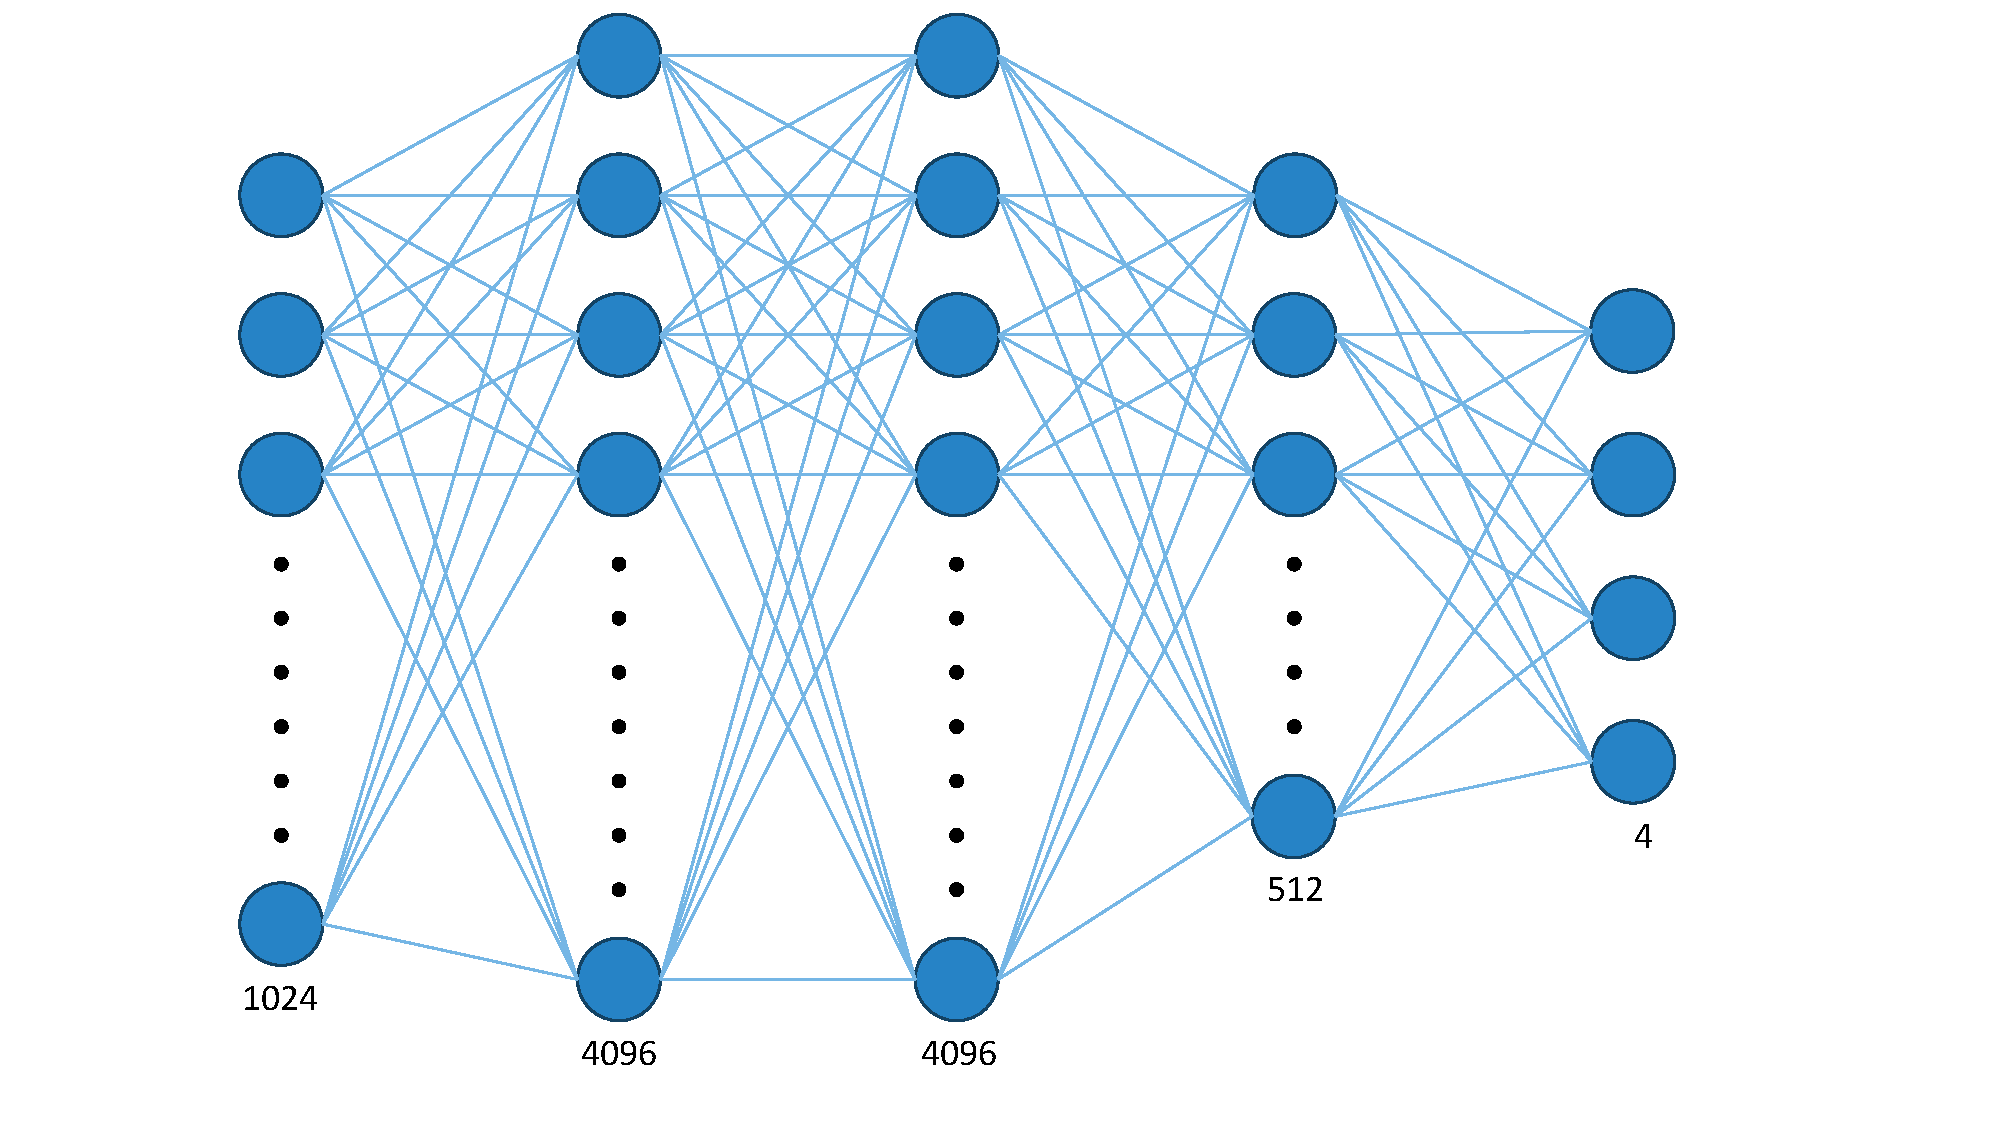
\includegraphics[width=.8\linewidth]{figures/spp/pose_net_diagram.pdf}
  \caption[Pose Regression Network]{Pose regression network taking a 1024 dimensional 
  input and providing a 4 dimensional output (three rotational parameters and a \( z \) coordinate).}
~\label{figure:spp_pose_block}
\end{figure}

It is not necessary to regress the entire 6DoF pose directly in the case of \textit{known} camera intrinsic 
parameters. For a given depth value \( z \), the \( x \) and \( y \) coordinates of a detected object may 
be recovered as follows in Equations~\ref{eqn:spp_x_3d} and~\ref{eqn:spp_y_3d} by making use of the 2D bounding 
box coordinates regressed by the network, as in Section~\ref{subsub:spp_neural_rpn}.

To recover the 3D position of an object of interest, a simple camera unprojection may be performed. 
However, first the pixel coordinates of the object must be computed. Taking the object's \( x \) image 
location to be the centre of the \( x \) dimension of the bounding box, and the the \( y \) coordinate 
to be the bottom of the bounding box, the pixel coordinates may be computed as follows in 
Equations~\ref{eqn:spp_x_pred} and~\ref{eqn:spp_y_pred}, for some bounding box \( \bm{b} \).

\begin{equation}
  \label{eqn:spp_x_pred}
  \bar{x} = \bm{b}_{x}^{tl} + \frac{1}{2} \Big[ \bm{b}_{x}^{br} - \bm{b}_{x}^{tl} \Big]
\end{equation}

\begin{equation}
  \label{eqn:spp_y_pred}
  \bar{y} = \bm{b}_{y}^{br}
\end{equation}

Where in Equations~\ref{eqn:spp_x_pred} and~\ref{eqn:spp_y_pred}, the indices \( tl \) and \( br \) 
represent the top left and bottom right bounding box coordinates, respectively. Finally, the camera 
space \( x \) and \( y \) coordinates of the object of interest may be recovered as follows in 
Equations~\ref{eqn:spp_x_3d} and~\ref{eqn:spp_y_3d}.

\begin{equation}
  \label{eqn:spp_x_3d}
  x = \frac{z}{f_{x}} \Big[ \bar{x} - c_{x} \Big]
\end{equation}

\begin{equation}
  \label{eqn:spp_y_3d}
  x = \frac{z}{f_{y}} \Big[ \bar{y} - c_{y} \Big]
\end{equation}

\subsubsection{Latent Shape Space Regression Component}
~\label{subsub:spp_neural_latent}
As outlined in Section~\ref{sec:spp_algorithm}, the GPLVM component of the network provides 
a generative model over 3D shape for the object class of focus in this work. However, to draw 
a 3D shape from the GP distribution, the GP must be conditioned on a 2D latent space 
point. The purpose of the shape regression network is to regress, for a given feature map corresponding 
to an RoI, a latent space point on which the GP is conditioned to predict a 3D shape descriptor.

\begin{figure}[!htbp]
  \centering
  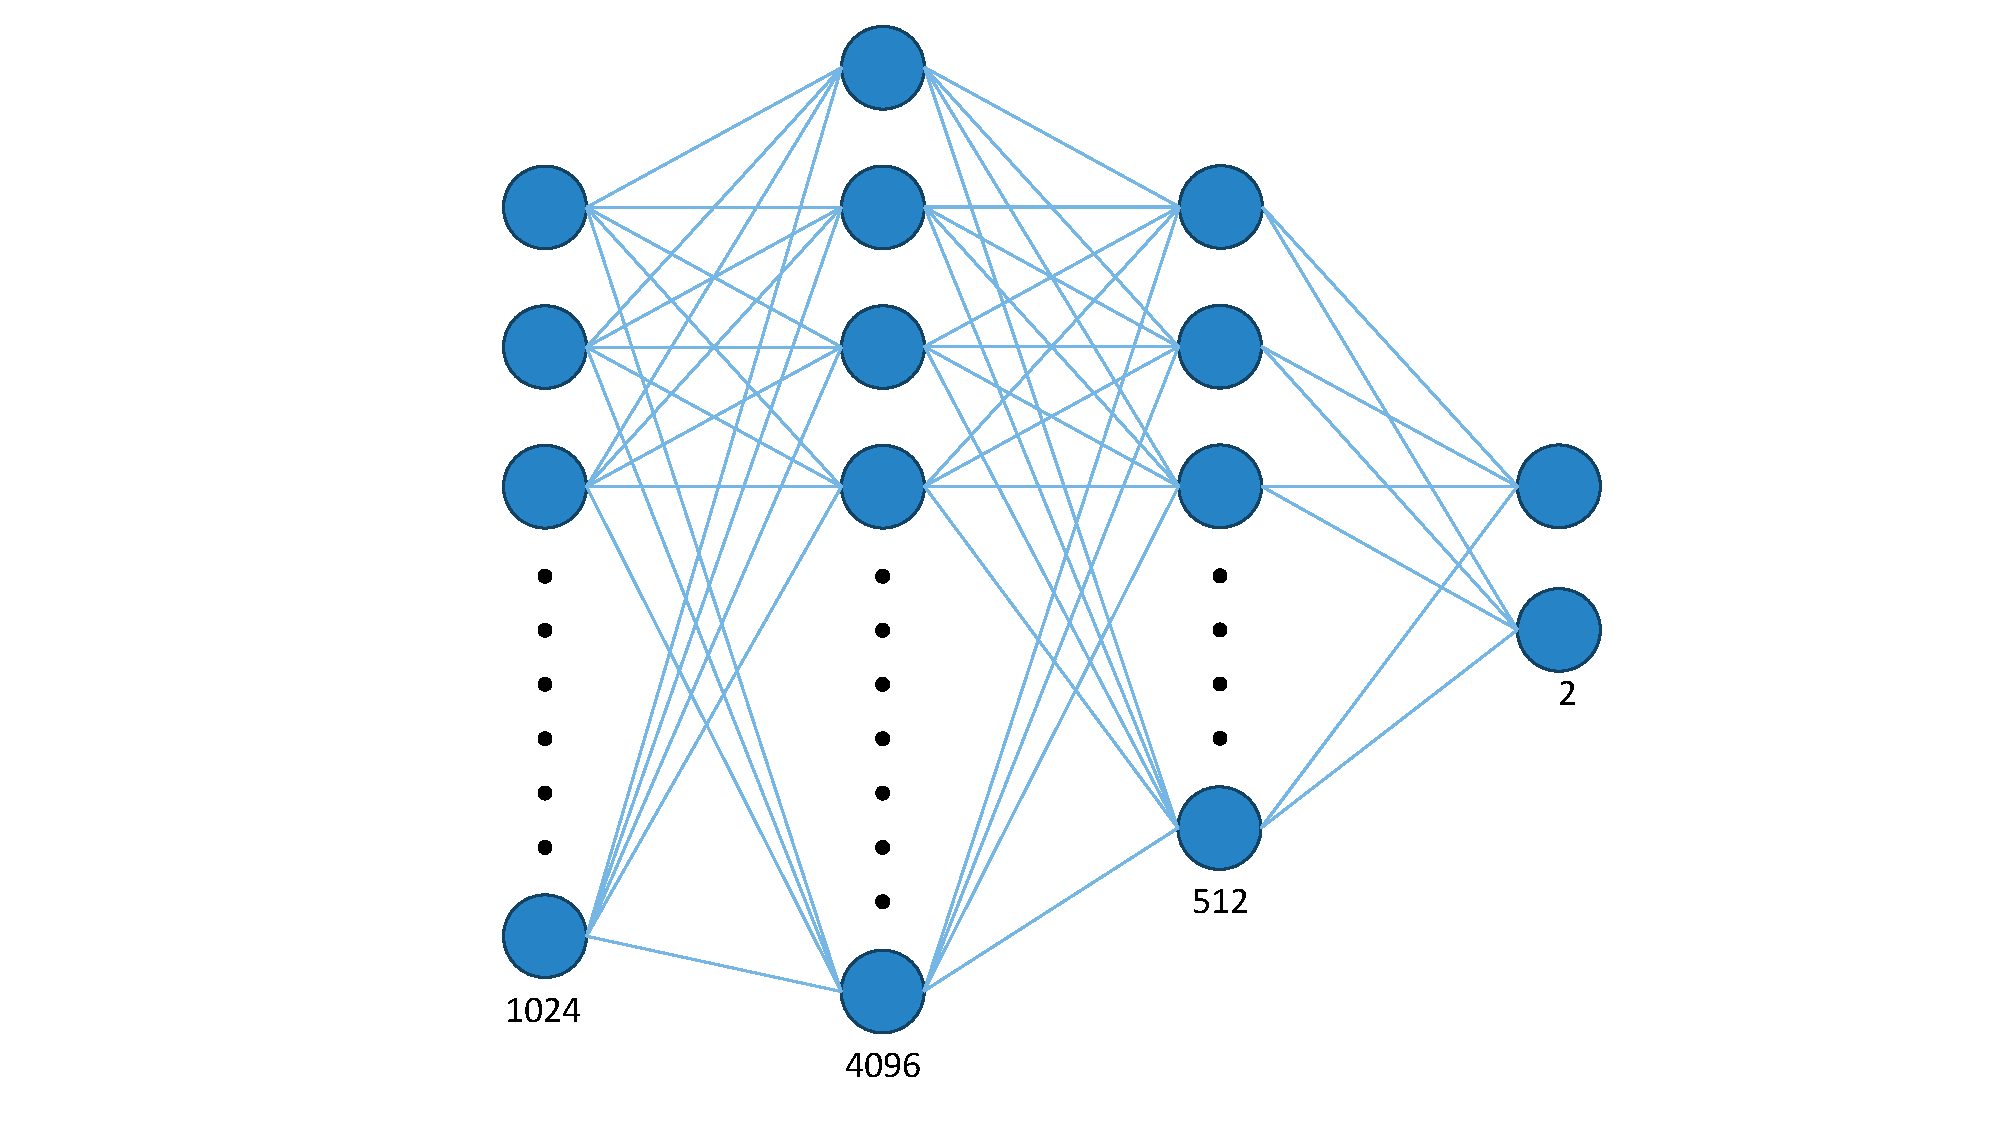
\includegraphics[width=.8\linewidth]{figures/spp/shape_net_diagram.pdf}
  \caption[Shape Regression Network]{Shape regression network taking a 1024 dimensional 
  input and providing a 2 dimensional output (a point in the latent shape space).}
~\label{figure:spp_shape_block}
\end{figure}

The topology of the shape network is analogous to the pose network of Section~\ref{subsub:spp_neural_pose}. 
Much like the pose network, the shape network consists of a set of linear transforms and nonlinear 
activations. The domain of the GP shape prior is \( [0, 1] \), so the two outputs of the shape network 
are given by the sigmoid activation function.

% TODO: Reorder this; goes from high level intro to GP's... bit heavy 
\section{Gaussian Process Latent Variable Model}
~\label{sec:spp_gplvm}
The use of a GPLVM for the embedding of 3D shape is motivated by the assumption that for a 
given category of object, cars for example, there is enough shared geometric structure that 
a comprehensive generative model may be formed. In the linear case, the GPLVM is equivalent 
to a probabilistic formulation of Principal Component Analysis (PCA), where a linear mapping 
from observed to hidden, latent space is derived. 

Under a Bayesian formulation, the often intractable latent variables pertaining to the linear 
mapping may be marginalised, such that the latent embedding itself may be optimised directly. The 
given framework allows for complex, non-linear embeddings to be learnt via the use of kernel functions, 
though the optimisation in this case is often non-convex and highly non-linear.

A GP may be viewed as a prior distribution over continuous functions. The posterior 
may be obtained by conditioning on observed data, to obtain a function estimate for each data point.
A visual example of a GP is given in Figure~\ref{figure:gp_func_dist}.
\begin{figure}[!htbp]
  \centering
  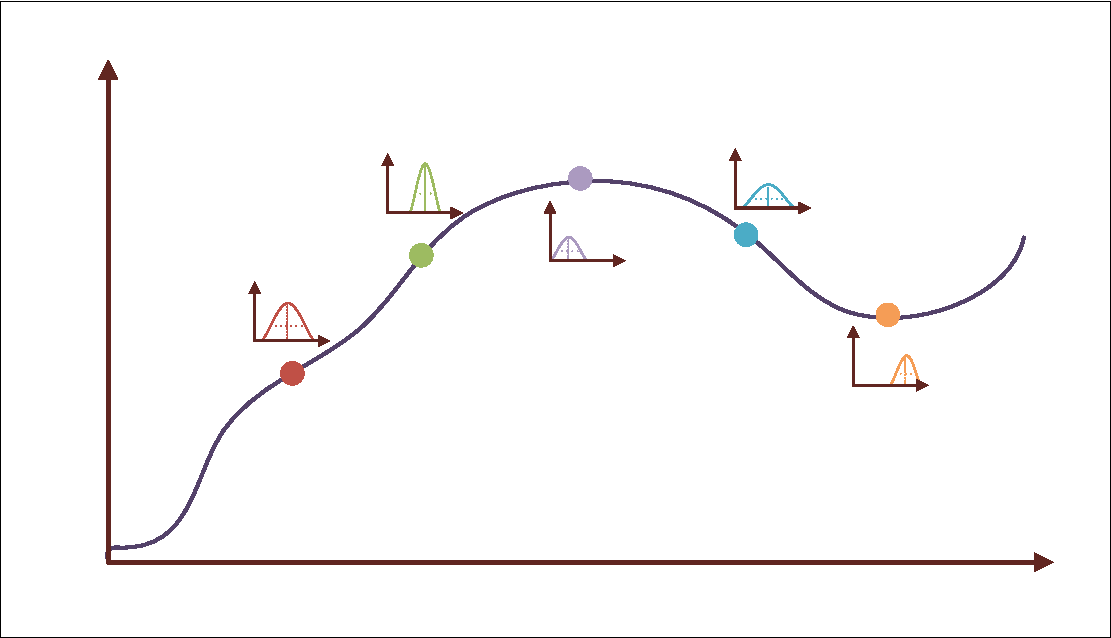
\includegraphics[width=\linewidth]{figures/spp/gp.pdf}
  \caption[GP as a Distribution Over Functions]{For each point along \( x \), 
  a function \( \bm{f} \sim \mathcal{GP}(\bm{\mu}, \bm{\Sigma}) \) drawn from a Gaussian Process 
  \( \mathcal{GP} \) is evaluated at \( x \).}
~\label{figure:gp_func_dist}
\end{figure}

\subsection{Gaussian Process Marginal Likelihood}
~\label{subsec:spp_gp_marginal_likelihood}
The first step is to define a latent variable model of the form given in Equation~\ref{eqn:spp_gp_lvm}.
\begin{equation}
  \label{eqn:spp_gp_lvm}
  P(\bm{Y} \given \bm{X}, \bm{W}, \beta) = P(\bm{Y} \given \bm{WX}^{T}, \beta^{-1}\bm{I})
\end{equation}
In Equation~\ref{eqn:spp_gp_lvm} the observed data \(\bm{Y} \in \mathbb{R}^{N \times D}\) 
is mapped to a lower dimensionality manifold \(\bm{X} \in \mathbb{R}^{N \times P}\), by parameters 
\(\bm{W} \in \mathbb{R}^{P \times D}\) and variance \( \beta \). In Equation~\ref{eqn:spp_gp_lvm}, 
the latent variable model \( P(\bm{Y} \given \bm{X}, \bm{W}, \beta) \) provides a linear mapping 
defined by the aforementioned latent variables \( \bm{W} \). As \( \bm{W} \) is unobservable and 
thus not directly tractable, it may be analytically marginalised out, given a suitable likelihood 
and prior. The marginal likelihood of \(\bm{X}\) is of the form outlined in Equation~\ref{eqn:spp_gp_marginal}.
\begin{equation}
  \label{eqn:spp_gp_marginal}
  P(\bm{Y} \given \bm{X}, \beta) = \int P(\bm{Y} \given \bm{X}, \bm{W}, \beta) P(\bm{W}) \intd{\bm{W}}
\end{equation}
In Equation~\ref{eqn:spp_gp_marginal}, \( P(\bm{Y} \given \bm{X}, \bm{W}, \beta) \) is of 
a multivariate Gaussian form and \(P(\bm{W})\) is a multivariate Gaussian conjugate prior of the 
form \(\mathcal{N}(\bm{W} \given \bm{0}, \bm{I})\).

To find the marginal distribution outlined in Equation~\ref{eqn:spp_gp_marginal}, it's form may 
first be simplified as follows in Equation~\ref{eqn:spp_gp_marginal_simplify}.
\begin{align}
  \label{eqn:spp_gp_marginal_simplify}
  % Line 1.
  P(\bm{Y} \given \bm{X}, \beta) ={}& \int \mathcal{N}(\bm{Y} \given \bm{WX}^{T}, \beta^{-1}\bm{I})
  \mathcal{N}(\bm{W} \given \bm{0}, \bm{I}) \intd{\bm{W}} \\
  % Line 2.
  ={}& \int \frac{1}{\sqrt{\left|2\pi\beta^{-1}\bm{I}\right|}} e^{ 
    -\frac{\beta}{2} {\big( \bm{Y} - \bm{WX} \big)}^{T} \big( \bm{Y} - \bm{WX} \big) 
  }
  \frac{1}{\sqrt{\left|2\pi\bm{I}\right|}} e^{ 
    -\frac{1}{2} \bm{W}^{T}\bm{W}} \intd{\bm{W}} \\
  % Line 3.
  ={}& \frac{1}{\sqrt{\left|2\pi\beta^{-1}\bm{I}\right|}} \frac{1}{\sqrt{\left|2\pi\bm{I}\right|}} 
  \int e^{
    -\frac{\beta}{2} {\big( \bm{Y} - \bm{WX} \big)}^{T} \big( \bm{Y} - \bm{WX} \big) 
    -\frac{1}{2} \bm{W}^{T}\bm{W}} \intd{\bm{W}} \\
  % Line 4.
  \propto& \int e^{
    -\frac{\beta}{2} {\big( \bm{Y} - \bm{WX} \big)}^{T} \big( \bm{Y} - \bm{WX} \big) 
    -\frac{1}{2} \bm{W}^{T}\bm{W}} \intd{\bm{W}} \\
  % Line 5.
  \propto& \int e^{ 
  -\frac{1}{2} \Big[
    \beta {\big( \bm{Y} - \bm{X}^{T}\bm{W} \big)}^{T} \big( \bm{Y} - \bm{X}^{T}\bm{W} \big) 
    + \bm{W}^{T}\bm{W}
  \Big]} \intd{\bm{W}} \\
  % Line 6.
  \propto& e^{ -\frac{\beta}{2} \bm{Y}^{T}\bm{Y}} 
  \int e^{
  -\frac{1}{2} \Big[
    -\beta \big( \bm{Y}^{T}\bm{X}^{T}\bm{W} \big) 
    -\beta {\big( \bm{W}^{T}\bm{XY} \big)}^{T}
    +\beta \bm{W}^{T}\bm{XX}^{T}\bm{W}
    + \bm{W}^{T}\bm{W}\Big]} \intd{\bm{W}} \\
  % Line 7.
  \propto& e^{-\frac{\beta}{2} \bm{Y}^{T}\bm{Y}} 
  \int e^{
  -\frac{1}{2} \Big[
    -2\beta \bm{Y}^{T}\bm{X}^{T}\bm{W}
    +\beta \bm{W}^{T}\bm{XX}^{T}\bm{W}
    + \bm{W}^{T}\bm{W}
  \Big]} \intd{\bm{W}} \\
  % Line 7.
  \propto& e^{-\frac{\beta}{2} \bm{Y}^{T}\bm{Y}} 
  \int e^{
  -\frac{1}{2} \Big[
    \bm{W}^{T} \big( \beta \bm{XX}^{T} + \bm{I} \big) \bm{W}
    -2\beta \bm{Y}^{T}\bm{X}^{T}\bm{W}
  \Big]} \intd{\bm{W}}
\end{align}

To make the integral over \(\bm{W}\) tractable in Equation~\ref{eqn:spp_gp_marginal_simplify}, 
the distribution \(P(\bm{Y} \given \bm{X}, \beta)\) must be a Gaussian; an exponential 
of a quadratic form. Completing the square in \(\bm{W}\) allows the marginal to be expressed 
in such a form. First, a change of variables is made, as in Equation~\ref{eqn:spp_gp_marginal_change}.
\begin{align}
  \label{eqn:spp_gp_marginal_change}
  \bm{A} ={}& \beta \bm{XX}^{T} + \bm{I}\\
  \bm{b} ={}& \beta \bm{Y}^{T} \bm{X}^{T}
\end{align}

The procedure to integrate over \( \bm{W} \) and transform \( P(\bm{Y} \given \bm{X}, \beta) \) 
into a valid multivariate Gaussian form is as follows in Equation~\ref{eqn:spp_gp_complete}.
\begin{align}
  \label{eqn:spp_gp_complete}
  % Line 1.
  P(\bm{Y} \given \bm{X}, \beta) \propto{}& e^{-\frac{\beta}{2}\bm{Y}^{T}\bm{Y}}
  \int e^{-\frac{1}{2} 
  \big[
    \bm{W}^{T}\bm{AW} - 2\bm{bW}  
  \big]} \intd{\bm{W}}\\
  % Line 2.
  \propto& e^{-\frac{\beta}{2}\bm{Y}^{T}\bm{Y}}
  \int e^{ 
    -\frac{1}{2} \bm{W}^{T}\bm{AW} 
    - 2\bm{bW} 
    - \bm{b}^{T}\bm{A}^{-1}\bm{b}} \intd{\bm{W}}\\
  % Line 3.
  \propto& e^{-\frac{\beta}{2}\bm{Y}^{T}\bm{Y}}
  \int e^{ 
    -\frac{1}{2} \bm{W}^{T}\bm{AW} 
    - 2\bm{bA}\bm{A}^{-1}\bm{W}
    + \bm{b}^{T}\bm{A}^{-1}\bm{AA}^{-1}\bm{b}} \intd{\bm{W}}\\
  % Line 4.
  \propto& e^{-\frac{\beta}{2}\bm{Y}^{T}\bm{Y}}
  \int e^{-\frac{1}{2} \big[ 
      {\big( \bm{W} - \bm{A}^{-1}\bm{b} \big)}^{T}
      \bm{A}
      \big( \bm{W} - \bm{A}^{-1}\bm{b} \big)
      - \bm{b}^{T}\bm{A}^{-1}\bm{b}
    \big]} \intd{\bm{W}}\\
  % Line 5.
  \propto& e^{-\frac{\beta}{2}\bm{Y}^{T}\bm{Y}}
  e^{-\frac{1}{2} \big[
      \sqrt{\left| 2 \pi \bm{A} \right|}
      - \bm{b}^{T}\bm{A}^{-1}\bm{b}
    \big]}\\
  % Line 6.
  \propto& e^{\frac{1}{2} \big[
    \beta \bm{Y}^{T} \beta \bm{Y}
    - \bm{b}^{T}\bm{A}^{-1}\bm{b}
    \big]}\\
  % Line 7.
  \propto& e^{-\frac{1}{2}
  \bm{Y}^{T} \big(
    \beta \bm{I} - \beta^{2}\bm{X}^{T}\bm{A}^{-1}\bm{X}
    \big)\bm{Y}}
\end{align}

With the distribution \(P(\bm{Y} \given \bm{X}, \beta)\) derived as being proportional to  
an exponentiated quadratic form as in Equation~\ref{eqn:spp_gp_complete}, it is 
clear that the inverse covariance matrix \(\bm{\Sigma}^{-1}\) of the Gaussian distribution 
corresponding to \(P(\bm{Y} \given \bm{X}, \beta)\) is as follows in Equation~\ref{eqn:spp_sig_inv}.
\begin{align}
  \label{eqn:spp_sig_inv}
  % Line 1.
  \bm{\Sigma}^{-1} ={}& \beta \bm{I} - \beta^{2} \bm{X}^{T} \bm{A}^{-1} \bm{X}\\
  % Line 2.
  ={}& \beta \bm{I} - \beta^{2} \bm{X}^{T} {\big(\beta \bm{XX}^{T} + \bm{I} \big)}^{-1}
\end{align}

To obtain the covariance matrix of the distribution \(P(\bm{Y} \given \bm{X}, \beta)\), the 
form of it's inverse may be simplified by the use of the matrix inversion lemma (also known 
as the Woodbury Identity)~\cite{GPML}. First making a change of variables in the Woodbury Identity 
as in Equation~\ref{eqn:spp_sig_inv_w}.
\begin{align}
  % Variable change.
  \label{eqn:spp_sig_inv_w}
    \bm{A} ={}& \beta^{-1}\bm{I}\\
    \bm{C} ={}& \bm{I}\\
    \bm{U} ={}& \bm{X}^{T}\\
    \bm{V} ={}& \bm{X}
  \shortintertext{in}
  % Woodbury.
  (\bm{A} + \bm{UCV}) ={}&
  \bm{A}^{-1} - \bm{A}^{-1}\bm{U} 
  {(\bm{C}^{-1} + \bm{VA}^{-1}\bm{U})}^{-1}
  \bm{VA}^{-1}
\end{align}

The simplified form of \( \bm{\Sigma}^{-1} \) is thus given as follows in 
Equation~\ref{eqn:spp_sig_inv_simp}.
\begin{align}
  \label{eqn:spp_sig_inv_simp}
  % Line 1.
  \bm{\Sigma}^{-1} ={}& \beta \bm{I} - \beta^{2} \bm{X}^{T} 
  {\big(\beta \bm{XX}^{T} + \bm{I} \big)}^{-1}\\
  % Line 2.
  ={}& \beta^{-1} \bm{I} + \bm{X}^{T}\bm{X}
\end{align}

It follows from Equation~\ref{eqn:spp_sig_inv_simp}, that the covariance matrix \( \bm{\Sigma} \)
takes the form of Equation~\ref{eqn:spp_sig}.
\begin{align}
  \label{eqn:spp_sig}
  % Line 1.
  \bm{\Sigma} ={}& {(\bm{\Sigma}^{-1})}^{-1}\\
  % Line 2.
  ={}& \bm{X}^{T}\bm{X} + \beta^{-1}\bm{I}
\end{align}

As such, the form of the normalized marginal likelihood \(P(\bm{Y} \given \bm{X}, \beta)\) of 
\( \bm{W} \) is given in Equation~\ref{eqn:spp_gp_marginal_simp}.
\begin{equation}
  \label{eqn:spp_gp_marginal_simp}
  P(\bm{Y} \given \bm{X}, \beta) = \mathcal{N}(\bm{Y} \given \bm{0}, 
  \bm{X}^{T}\bm{X} + \beta^{-1} \bm{I})
\end{equation}

\subsection{Gaussian Process Fitting}
~\label{subsec:spp_gp_fitting}
As outlined in Section~\ref{sec:spp_gplvm}, the given formulation of the marginal likelihood 
in Equation~\ref{eqn:spp_gp_marginal_simp} can be optimised directly for the latent embedding 
\( \bm{X} \). For a mapping from \(\mathbb{R}^{N \times D} \) space to \(\mathbb{R}^{N \times P} \)
space (for \( P < D \)), the latent embedding \( \bm{X} \) may be initialized by applying an 
orthogonal linear transform to the observed data and reducing dimensionality. One such approach 
is to apply PCA to the observed data, taking the first \(P\) reverse sorted eigenvalues of the 
covariance matrix. Additionally, in the non-linear case, where the covariance matrix \( \bm{\Sigma} \) 
is generated by a given kernel function \( \bm{\kappa} \), the hyperparameters of \( \bm{\kappa} \) may 
also be optimised.

To find the most probable latent space embedding, the latent variables \( \bm{X} \) may be 
found by directly optimising the marginal likelihood of Equation~\ref{eqn:spp_gp_marginal_simp}. 
As such, the natural logarithm may also be optimised for the latent variables \( \bm{X} \) and 
is given in Equation~\ref{eqn:spp_gp_marginal_log}.
\begin{align}
  \label{eqn:spp_gp_marginal_log}
  % Line 1.
  \mathcal{L} ={}& -\frac{DN}{2} \ln(2\pi)
  -\frac{D}{2} \ln(\left| \bm{\Sigma} \right|)
  -\frac{1}{2} \text{tr}(\bm{\Sigma}^{-1} \bm{YY}^{T})\\
  % Line 2.
  ={}& -\frac{DN}{2} \ln(2\pi)
  -\frac{D}{2} \ln(\left| \bm{\Sigma} \right|)
  -\frac{1}{2} \bm{Y}^{T}\bm{\Sigma}\bm{Y}
\end{align}

The gradient of the log marginal of Equation~\ref{eqn:spp_gp_marginal_log} 
is derived as follows in Equation~\ref{eqn:spp_gp_log_marginal_grad}.
\begin{align}
  \label{eqn:spp_gp_log_marginal_grad}
  % Line 1.
  \frac{\partial \mathcal{L}}{\partial \bm{X}} ={}&
  -\frac{1}{2} \Bigg[
    \Big( D \frac{\partial}{\partial \bm{\Sigma}} 
    \ln \big( \left| \bm{\Sigma} \right| \big) \Big) 
    \frac{\partial \bm{\Sigma}}{\partial \bm{X}}
    + \Big( \frac{\partial}{\partial \bm{\Sigma}}
    \bm{Y}^{T} \bm{\Sigma}^{-1} \bm{Y} \Big)
    \frac{\partial \bm{\Sigma}}{\partial \bm{X}}
  \Bigg]\\
  % Line 2.
  ={}& -\frac{1}{2} \Bigg[
    D \bm{\Sigma}^{-1} \frac{\partial \bm{\Sigma}}{\partial \bm{X}}
    - \bm{\Sigma}^{-1} \bm{YY}^{T} \bm{\Sigma}^{-1} 
    \frac{\partial \bm{\Sigma}}{\partial \bm{X}}
  \Bigg]\\
  % Line 3.
  ={}& -\frac{1}{2} \Bigg[
    D \bm{\Sigma}^{-1} 2 \bm{X}
    - \bm{\Sigma}^{-1} \bm{YY}^{T} \bm{\Sigma}^{-1} 2 \bm{X}
  \Bigg]\\
  % Line 4.
  ={}& -D \bm{\Sigma}^{-1} \bm{X}
  + \bm{\Sigma}^{-1} \bm{YY}^{T} \bm{\Sigma}^{-1} \bm{X}
\end{align}

The gradient derived in Equation~\ref{eqn:spp_gp_log_marginal_grad} holds 
for the case when \( \bm{\Sigma} = \bm{X}^{T}\bm{X} + \beta^{-1} \bm{I} \). 
However, for \( \bm{\Sigma} = \bm{\kappa}(.) \) where \( \bm{\kappa} \) is 
a given kernel function, the result of the derivation of Equation
~\ref{eqn:spp_gp_log_marginal_grad} is applicable. When substituting 
\( \frac{\partial \bm{\Sigma}}{\partial \bm{X}} \) with 
\( \frac{\partial \bm{\kappa}}{\partial \bm{X}} \), the gradient is thus 
given in Equation~\ref{eqn:spp_gp_log_marginal_grad_kernel}.
\begin{equation}
  \label{eqn:spp_gp_log_marginal_grad_kernel}
  \frac{\partial \mathcal{L}}{\partial \bm{X}} = 
  -\frac{1}{2} \Bigg[
    D \bm{\Sigma}^{-1} \frac{\partial \bm{\kappa}}{\partial \bm{X}}
    - \bm{\Sigma}^{-1} \bm{YY}^{T} \bm{\Sigma}^{-1} 
    \frac{\partial \bm{\kappa}}{\partial \bm{X}}
  \Bigg]
\end{equation}

It should be noted that the gradient \( \frac{\partial \bm{\kappa}}{\partial \bm{X}} \)
may also be substituted for \( \frac{\partial \bm{\kappa}}{\partial \theta} \), for 
some hyperparameter \( \theta \) of a given kernel \( \bm{\kappa} \). A common non-linear covariance 
kernel function in the GP literature is the exponentiated quadratic~\cite{Lawrence2005}, which takes 
the form given in Equation~\ref{eqn:spp_exp_quad}.
\begin{align}
  \label{eqn:spp_exp_quad}
  % Line 1.
  \bm{\kappa} \big( \bm{x}_{i}, \bm{x}_{j}, \theta_{0}, 
  \theta_{1}, \theta_{2}, \lambda \big) ={}&
  \theta_{0} e^{-\frac{\lambda}{2} 
  \left\lVert \bm{x}_{i} - \bm{x}_{j} \right\rVert^{2}}
  + \theta_{1} + \theta_{2} \delta \big( -\frac{\lambda}{2} 
  \left\lVert \bm{x}_{i} - \bm{x}_{j} \right\rVert^{2} \big)\\
  % Line 2.
  ={}& \theta_{0} e^{-\frac{\lambda}{2} 
  \sum_{n}^{D} {\big( \bm{x}_{i, n} - \bm{x}_{j, n} \big)}^{2}}
  + \theta_{1} + \theta_{2} \delta \big( -\frac{\lambda}{2} 
  \sum_{n}^{D} {\big( \bm{x}_{i, n} - \bm{x}_{j, n} \big)}^{2} \big)
\end{align}

The gradient of the Exponentiated Quadratic kernel of Equation~\ref{eqn:spp_exp_quad},
\( \frac{\partial \bm{\kappa}}{\partial \bm{x}_{i, n}} \) for the \( n^{th} \) variable 
of \( \bm{x}_{i} \) can be derived as follows in Equation~\ref{eqn:exp_quad_grad_x}.
\begin{align}
  \label{eqn:exp_quad_grad_x}
  % Line 1.
  \frac{\partial \bm{\kappa}}{\partial \bm{x}_{i, n}} ={}& 
  \frac{\partial}{\partial \bm{x}_{i, n}} \theta_{0} e^{-\frac{\lambda}{2} 
  \sum_{n = 0}^{D} -\frac{\lambda}{2} {\big( \bm{x}_{i, n} - \bm{x}_{j, n} \big)}^{2}}\\
  % Line 2.
  ={}& \frac{\partial}{\partial \bm{x}_{i, n}} \theta_{0} e^{-\frac{\lambda}{2} 
  \sum_{n = 0}^{D} {\big( \bm{x}_{i, n} - \bm{x}_{j, n} \big)}^{2}} 
  \frac{\partial}{\partial \bm{x}_{i, n}} \sum_{n = 0}^{D} -\frac{\lambda}{2} 
  {\big( \bm{x}_{i, n} - \bm{x}_{j, n} \big)}^{2}\\
  % Line 3.
  ={}& \theta_{0} e^{-\frac{\lambda}{2} 
  \sum_{n = 0}^{D} {\big( \bm{x}_{i, n} - \bm{x}_{j, n} \big)}^{2}} 
  \frac{\partial}{\partial \bm{x}_{i, n}} \sum_{n = 0}^{D} -\frac{\lambda}{2} 
  {\big( \bm{x}_{i, n} - \bm{x}_{j, n} \big)}^{2}\\
  % Line 4.
  ={}& \lambda \theta_{0} e^{-\frac{\lambda}{2} 
  \sum_{n = 0}^{D} {\big( \bm{x}_{i, n} - \bm{x}_{j, n} \big)}^{2}} 
  {\big( \bm{x}_{i, n} - \bm{x}_{j, n} \big)}
\end{align}

Following the derivation of Equation~\ref{eqn:exp_quad_grad_x}, the remaining 
gradients of \( \kappa(.) \) may be trivially derived, as in Equation
~\ref{eqn:exp_quad_grad_rest}.
\begin{align}
  \label{eqn:exp_quad_grad_rest}
  % Line 1.
  \frac{\partial \bm{\kappa}}{\partial \bm{x}_{j, n}} ={}& 
  -\frac{\partial \bm{\kappa}}{\partial \bm{x}_{i, n}}\\
  % Line 2.
  \frac{\partial \bm{\kappa}}{\partial \theta_{0}} ={}&
  e^{-\frac{\lambda}{2} 
  \sum_{n = 0}^{D} {\big( \bm{x}_{i, n} - \bm{x}_{j, n} \big)}^{2}}\\
  % Line 3.
  \frac{\partial \bm{\kappa}}{\partial \theta_{1}} ={}& 1\\
  % Line 4.
  \frac{\partial \bm{\kappa}}{\partial \theta_{2}} ={}& 0\\
  % Line 5.
  \frac{\partial \bm{\kappa}}{\partial \lambda} ={}& 
  -\frac{1}{2} \sum_{n = 0}^{D} \theta_{0} {\big( \bm{x}_{i, n} - \bm{x}_{j, n} \big)}^{2}
  e^{-\frac{\lambda}{2} 
  \sum_{n = 0}^{D} {\big( \bm{x}_{i, n} - \bm{x}_{j, n} \big)}^{2}}
\end{align}

\section{Latent Space Shape Estimation}
~\label{sec:spp_latent_shape_est}
The form of the model outlined in Section~\ref{subsec:spp_gp_marginal_likelihood},
when trained as outlined in Section~\ref{subsec:spp_gp_fitting}, defines a GP prior 
over the latent space embedding \( \bm{X} \). When regressing a DCT compressed 3D shape, it is 
necessary to condition the DCT compressed 3D shape of a given latent space point on the GP prior. 
This conditioning yields a posterior mean estimation over 3D shape for a given latent space point.

The estimated posterior mean provides a Discrete Cosine Transform (DCT) compressed representation 
of an SDF shape volume \( \bm{\Phi} \in \mathbb{R}^{N \times N \times N} \). The DCT compressed form 
of \( \bm{\Phi} \) given by the aforementioned posterior mean is obtained by GP regression~\cite{GPML}. 
Finally, the true, uncompressed form of \( \bm{\Phi} \) is obtained by taking the IDCT of the posterior mean. 
The granularity of the geometric properties captured by the GP shape prior is governed by the number of DCT 
harmonics used in the compression and decompression processes at training and prediction.

\subsection{Shape Posterior Mean Estimation}
~\label{subsec:spp_pos_mean_est}
With the optimised latent variables \( \bm{X} \), the formulation outlined in 
Equation~\ref{eqn:spp_gp_marginal_simp} defines a GP prior 
over functions of \( \bm{X} \), as follows.
\begin{equation}
  \label{eqn:gp_prior}
  \bm{f}(\bm{X}) \sim \mathcal{GP}(\bm{0}, \bm{\Sigma}_{\bm{XX}})
\end{equation}

A GP prior may similarly be constructed for observed latent 
space points \( \bm{L} \), as follows.
\begin{equation}
  \label{eqn:gp_prior_latent}
  \bm{f}^{\star}(\bm{l}) \sim \mathcal{GP}(\bm{0}, \bm{\Sigma}_{\bm{LL}})
\end{equation}

It follows from Equations~\ref{eqn:gp_prior} and~\ref{eqn:gp_prior_latent} that 
the joint distribution over \( \bm{X} \) and \( \bm{L} \) can be formulated as 
follows in Equation~\ref{eqn:spp_gp_joint}.
\begin{equation}
  \label{eqn:spp_gp_joint}
  \begin{bmatrix}
    \bm{f}\\
    \bm{f}^{\star}
  \end{bmatrix}
  \sim \mathcal{N} \Bigg(
    \begin{bmatrix}
      \bm{0}\\
      \bm{0}
    \end{bmatrix},
    \begin{bmatrix}
      \bm{\Sigma}_{\bm{XX}} & \bm{\Sigma}_{\bm{XL}}\\
      \bm{\Sigma}_{\bm{LX}} & \bm{\Sigma}_{\bm{LL}}
    \end{bmatrix}
  \Bigg)
\end{equation}

The posterior of \( \bm{f}^{\star} \) conditioned on \( \bm{f} \) is given by
the distribution in Equation~\ref{eqn:spp_gp_conditional}.
\begin{equation}
  \label{eqn:spp_gp_conditional}
  P(\bm{f}^{\star} \given \bm{X}, \bm{L}, \bm{f}) = 
  \mathcal{N} \Big(
    \bm{\Sigma}_{LX} \bm{\Sigma}_{XX}^{-1} \bm{f}, 
    \bm{\Sigma}_{LL} - \bm{\Sigma}_{LX} \bm{\Sigma}_{XX}^{-1} \bm{\Sigma}_{XL}
  \Big) 
\end{equation}

As such, to obtain a posterior mean prediction for a latent space point \( \bm{l} \), 
a draw from the distribution outlined in Equation~\ref{eqn:spp_gp_conditional} is 
taken as follows in Equation~\ref{eqn:spp_gp_posterior_draw}.
\begin{equation}
  \label{eqn:spp_gp_posterior_draw}
  \bm{f}^{\star} \sim P(\bm{f}^{\star} \given \bm{X}, \bm{L}, \bm{f})
\end{equation}

Given the form of \( P(\bm{f}^{\star} \given \bm{X}, \bm{L}, \bm{f}) \) in Equation
~\ref{eqn:spp_gp_posterior_draw}, the posterior mean \( \bm{f}^{\star} \) and variance
\( \mathbb{V}^{\star} \) are given as follows in Equation~\ref{eqn:spp_mean_var}.
\begin{align}
  \label{eqn:spp_mean_var}
  % Line 1.
  \bm{f}^{\star} ={}& 
  \bm{\Sigma}_{\bm{XL}}^{T} \bm{\Sigma}_{\bm{XX}}^{-1} \bm{Y}\\
  % Line 2.
  \mathbb{\bm{f}^{\star}} ={}&
  \bm{\Sigma}_{\bm{LL}} - \bm{\Sigma}_{\bm{LL}}^{T} \bm{\Sigma}_{XL}^{-1} \bm{\Sigma}_{LL}
\end{align}

\subsection{Gaussian Process Posterior Mean Gradient}
~\label{subsec:gp_posterior_mean_grad}
Due to the gradient based optimisation of the approach outlined in this chapter, each 
component outlined in Figure~\ref{figure:spp_pipeline} must be differentiable. The formulation 
of the posterior mean of Equation~\ref{eqn:spp_mean_var} is differentiable with it's gradient 
derived as follows in Equation~\ref{eqn:spp_pos_mean_grad}.
\begin{align}
  \label{eqn:spp_pos_mean_grad}
  % Line 1.
  \frac{\partial \bm{f}^{\star}}{\partial \bm{L}} ={}&
  \frac{\partial}{\partial \bm{L}}
  \bm{\Sigma}_{\bm{XL}}^{T} \bm{\Sigma}_{\bm{XX}}^{-1} \bm{Y}\\
  % Line 2.
  ={}& \frac{\partial \bm{\Sigma}_{\bm{XL}}^{T}}{\partial \bm{L}}
  \bm{\Sigma}_{\bm{XX}}^{-1} \bm{Y}
  + \bm{\Sigma}_{\bm{XL}}^{T} 
  \frac{\partial\bm{\Sigma}_{\bm{XX}}^{-1}}{\partial \bm{L}} \bm{Y}
  + \bm{\Sigma}_{\bm{XL}}^{T} \bm{\Sigma}_{\bm{XX}}^{-1} 
  \frac{\partial \bm{Y}}{\partial \bm{L}}\\
  % Line 3.
  ={}& \frac{\partial \bm{\Sigma}_{\bm{XL}}^{T}}{\partial \bm{L}}
  \bm{\Sigma}_{\bm{XX}}^{-1} \bm{Y}
\end{align}

\subsection{Signed Distance Function Extraction}
~\label{subsec:sdf_extraction}
As outlined in Section~\ref{sec:spp_latent_shape_est}, the SDF volume \( \bm{\Phi} \) 
is generated by taking the IDCT of the posterior mean of the GP prior conditioned on 
a given latent space point, as given by Equation~\ref{eqn:spp_gp_conditional}. In the 
formulation presented in this work, the 2D latent point is generated by the shape 
network component following the RPN of Figure~\ref{figure:spp_pipeline}. 
The output of the shape network is constrained to the interval \( [0, 1] \) by the use 
of a sigmoid activation function.%TODO verify

The latent variable model outlined in Section~\ref{sec:spp_gplvm} is a distribution 
over a latent space embedding of 3D shape. However, the 3D shape data on which the GP 
prior is modelled is compressed with the DCT\@. The intuition behind the use of the DCT is 
the property that the number of harmonics used in the transform impacts on the granularity of 
the resultant 3D shape geometry. It has been shown~\cite{Ren2014} that the lower frequency 
harmonics of the DCT capture general structure and shape, whilst higher frequency harmonics 
capture finer detailed geometric features. An example of a decompressed SDF of a car is given 
in Figure~\ref{figure:spp_sdf_slices}.
\begin{figure}[!htbp]
  \centering
  \begin{tabular}{ccc}
    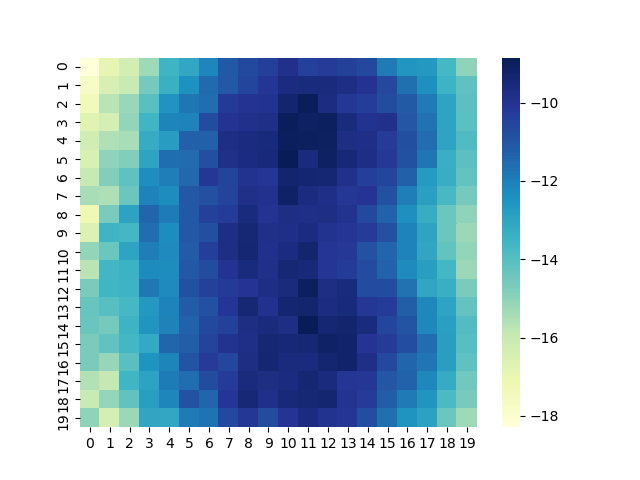
\includegraphics[width=.3\linewidth]{figures/spp/car_sdf_slices/x_0.png}&
		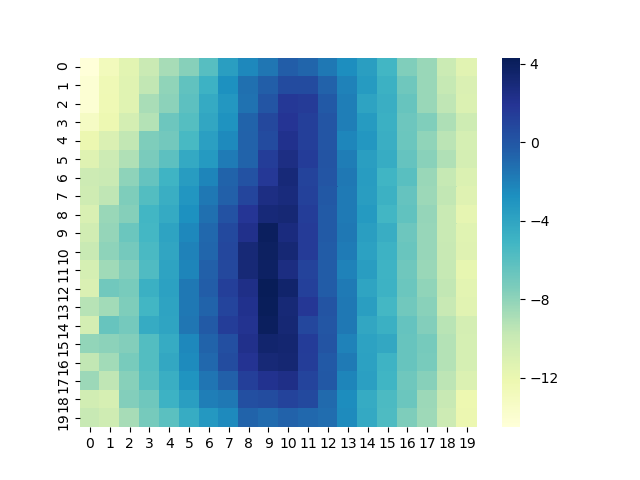
\includegraphics[width=.3\linewidth]{figures/spp/car_sdf_slices/x_10.png}&
		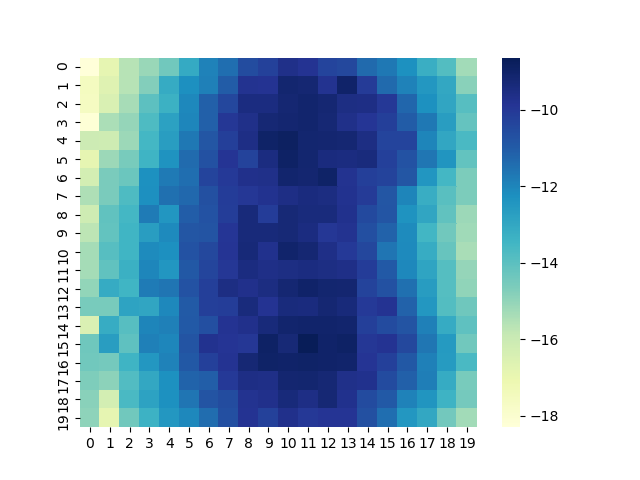
\includegraphics[width=.3\linewidth]{figures/spp/car_sdf_slices/x_19.png}\\
    (a) & (b) & (c) \\
    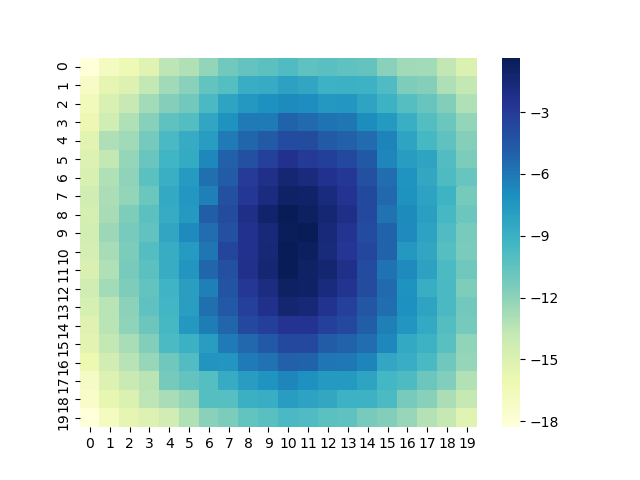
\includegraphics[width=.3\linewidth]{figures/spp/car_sdf_slices/y_0.png}&
		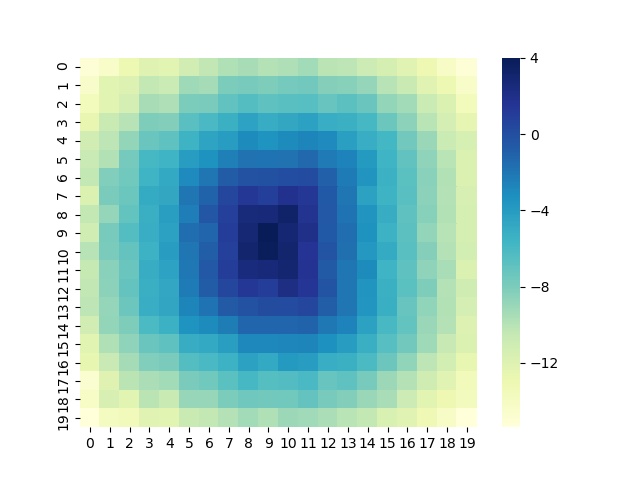
\includegraphics[width=.3\linewidth]{figures/spp/car_sdf_slices/y_10.png}&
		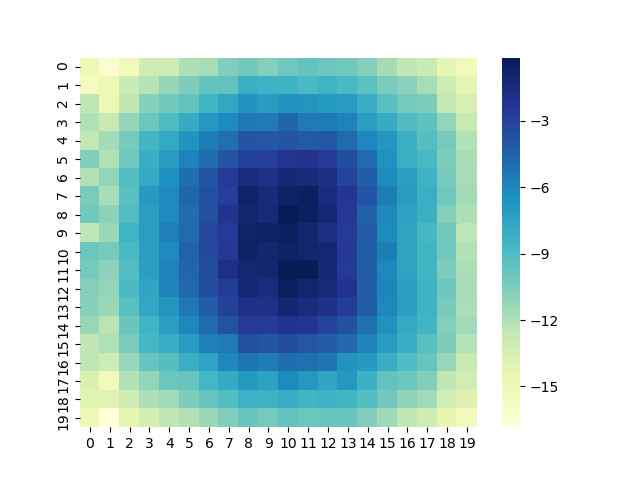
\includegraphics[width=.3\linewidth]{figures/spp/car_sdf_slices/y_19.png}\\
    (d) & (e) & (f) \\
    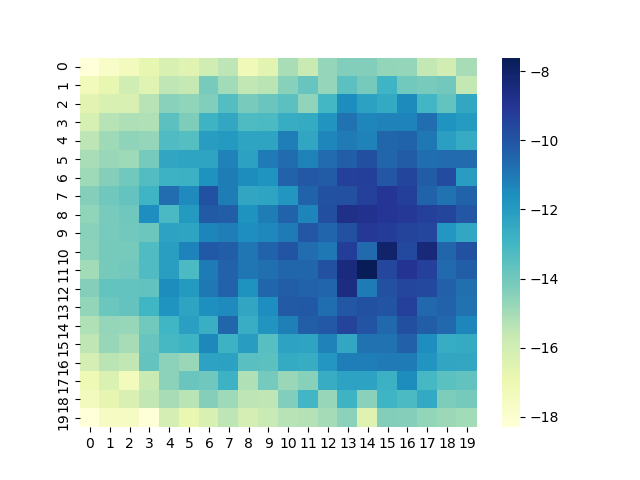
\includegraphics[width=.3\linewidth]{figures/spp/car_sdf_slices/z_0.png}&
		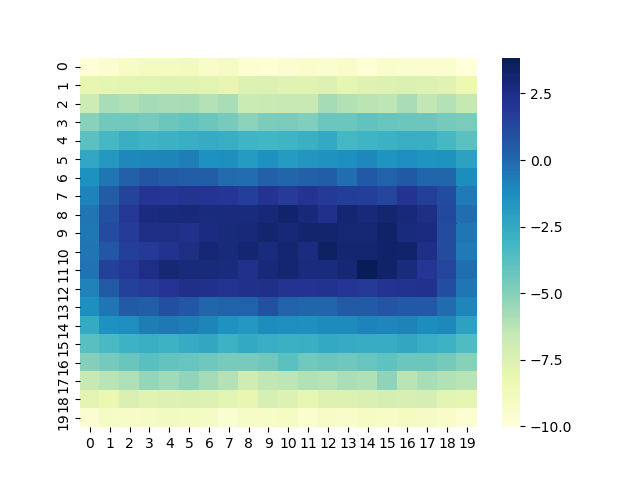
\includegraphics[width=.3\linewidth]{figures/spp/car_sdf_slices/z_10.png}&
		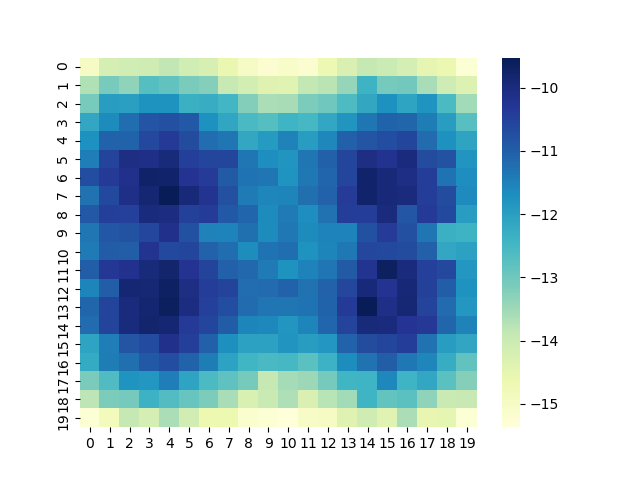
\includegraphics[width=.3\linewidth]{figures/spp/car_sdf_slices/z_19.png}\\
    (g) & (h) & (i)
  \end{tabular}
  \caption[SDF Slices Generated by DCT]
  {
    \begin{tabular}[t]{@{}l@{}}
      Slices of a Signed Distance Function embedding \( \bm{\Phi} \in \mathbb{R}^{20 \times 20 \times 20} \)
      of a\\ car at slices 0, 10 and 19:\\
      (a, b, c) Along the \(x\) axis.\\
      (d, e, f) Along the \(y\) axis.\\
      (g, h, i) Along the \(z\) axis.
    \end{tabular}
  }
~\label{figure:spp_sdf_slices}
\end{figure}

The voxels of an input SDF \( \bm{V} \) under the DCT (for model training) are thus given 
as follows in Equation~\ref{eqn:spp_dct}.
\begin{align}
  \label{eqn:spp_dct}
  % Line 1.
  \bm{\Psi}_{x, y, z} ={}& \bm{V}_{x, y, z} \Bigg[
  \sum_{x=0}^{N-1} \cos \Big[ \frac{\pi}{N} \big[ x + \frac{1}{2} \big] x \Big]
  \sum_{y=0}^{N-1} \cos \Big[ \frac{\pi}{N} \big[ y + \frac{1}{2} \big] y \Big]
  \sum_{z=0}^{N-1} \cos \Big[ \frac{\pi}{N} \big[ z + \frac{1}{2} \big] z \Big] \Bigg]\\
  % Line 2.
  ={}& \bm{V}_{x, y, z} \Bigg[
  \sum_{x=0}^{N-1} \cos \Big[ \frac{\pi \big( x^{2} + \frac{x}{2} \big)}{N} \Big]
  \sum_{y=0}^{N-1} \cos \Big[ \frac{\pi \big( y^{2} + \frac{y}{2} \big)}{N} \Big]
  \sum_{z=0}^{N-1} \cos \Big[ \frac{\pi \big( z^{2} + \frac{z}{2} \big)}{N} \Big] \Bigg]\\
  % Line 3.
  ={}& \sum_{x=0}^{N-1} \sum_{y=0}^{N-1} \sum_{z=0}^{N-1} \bm{V}_{x, y, z}
  \cos \Big[ \frac{\pi \big( x^{2} + \frac{x}{2} \big)}{N} \Big]
  \cos \Big[ \frac{\pi \big( y^{2} + \frac{y}{2} \big)}{N} \Big]
  \cos \Big[ \frac{\pi \big( z^{2} + \frac{z}{2} \big)}{N} \Big]
\end{align}

It follows that for a predicted posterior mean \( \bm{f}^{\star} \), as outlined in 
Equation~\ref{eqn:spp_gp_posterior_draw}, the voxels of the SDF corresponding to the 
estimation \( \bm{f}^{\star} \) may be extracted via the IDCT as follows in 
Equation~\ref{eqn:spp_idct}.
\begin{equation}
  \label{eqn:spp_idct}
  \bm{\Phi}_{x, y, z} = \sum_{x=0}^{N-1} \sum_{y=0}^{N-1} \sum_{z=0}^{N-1} 
  \bm{f}^{\star}_{x, y, z}
  \cos \Big[ \frac{\pi \big( x^{2} + \frac{x}{2} \big)}{N} \Big]
  \cos \Big[ \frac{\pi \big( y^{2} + \frac{y}{2} \big)}{N} \Big]
  \cos \Big[ \frac{\pi \big( z^{2} + \frac{z}{2} \big)}{N} \Big]
\end{equation}

An example of how the geometric detail of the decompressed model varies with the number 
of harmonics used, \( N \), is given in Figure~\ref{figure:spp_sdf_diff_harmonics}.
\begin{figure}[!htbp]
  \centering
  \begin{tabular}{ccc}
    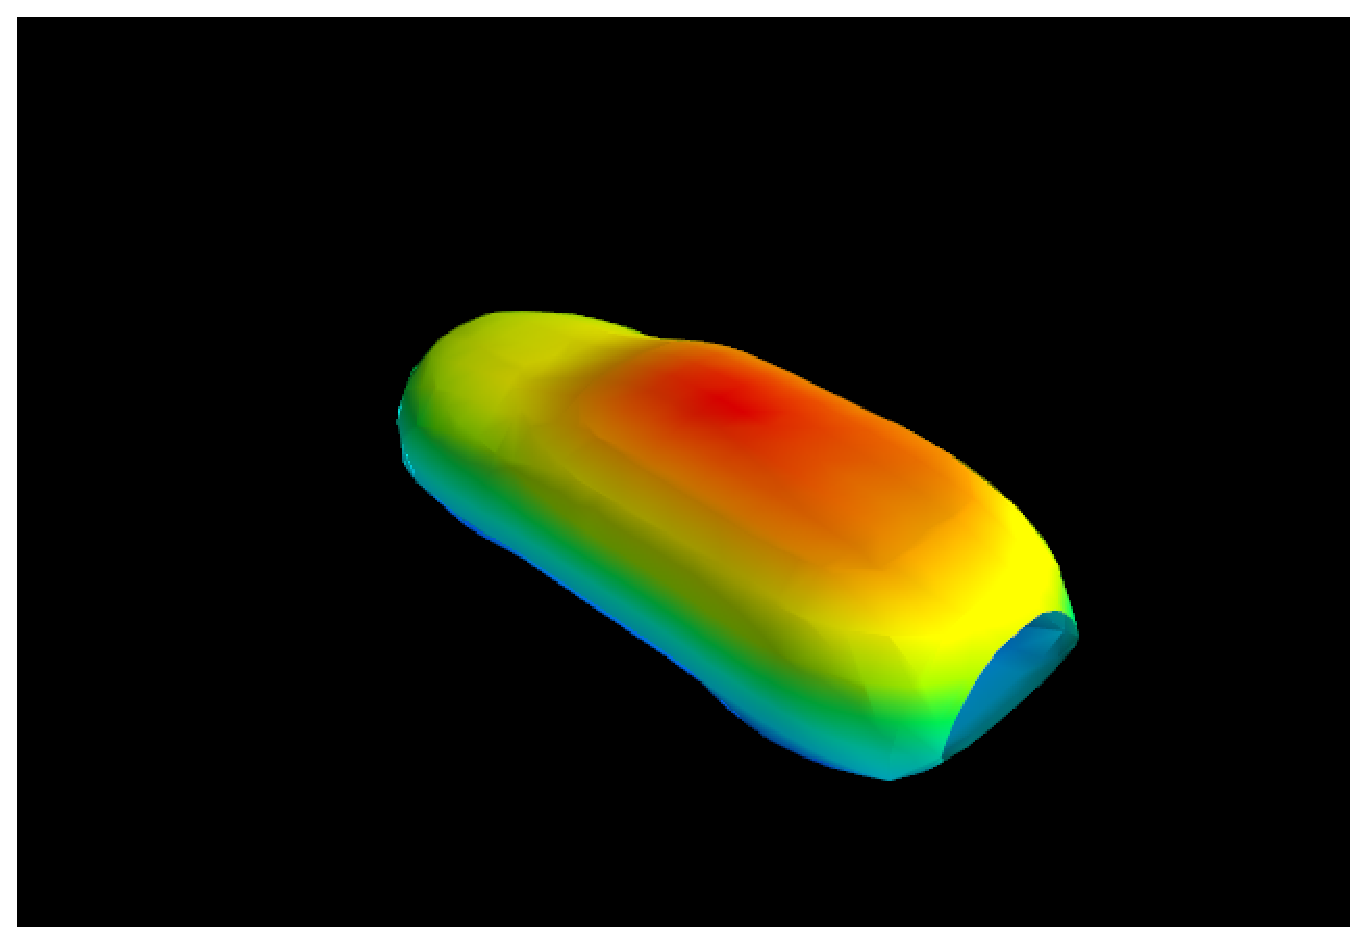
\includegraphics[width=.4\linewidth]{figures/spp/differing_harmonics/1.eps}&
		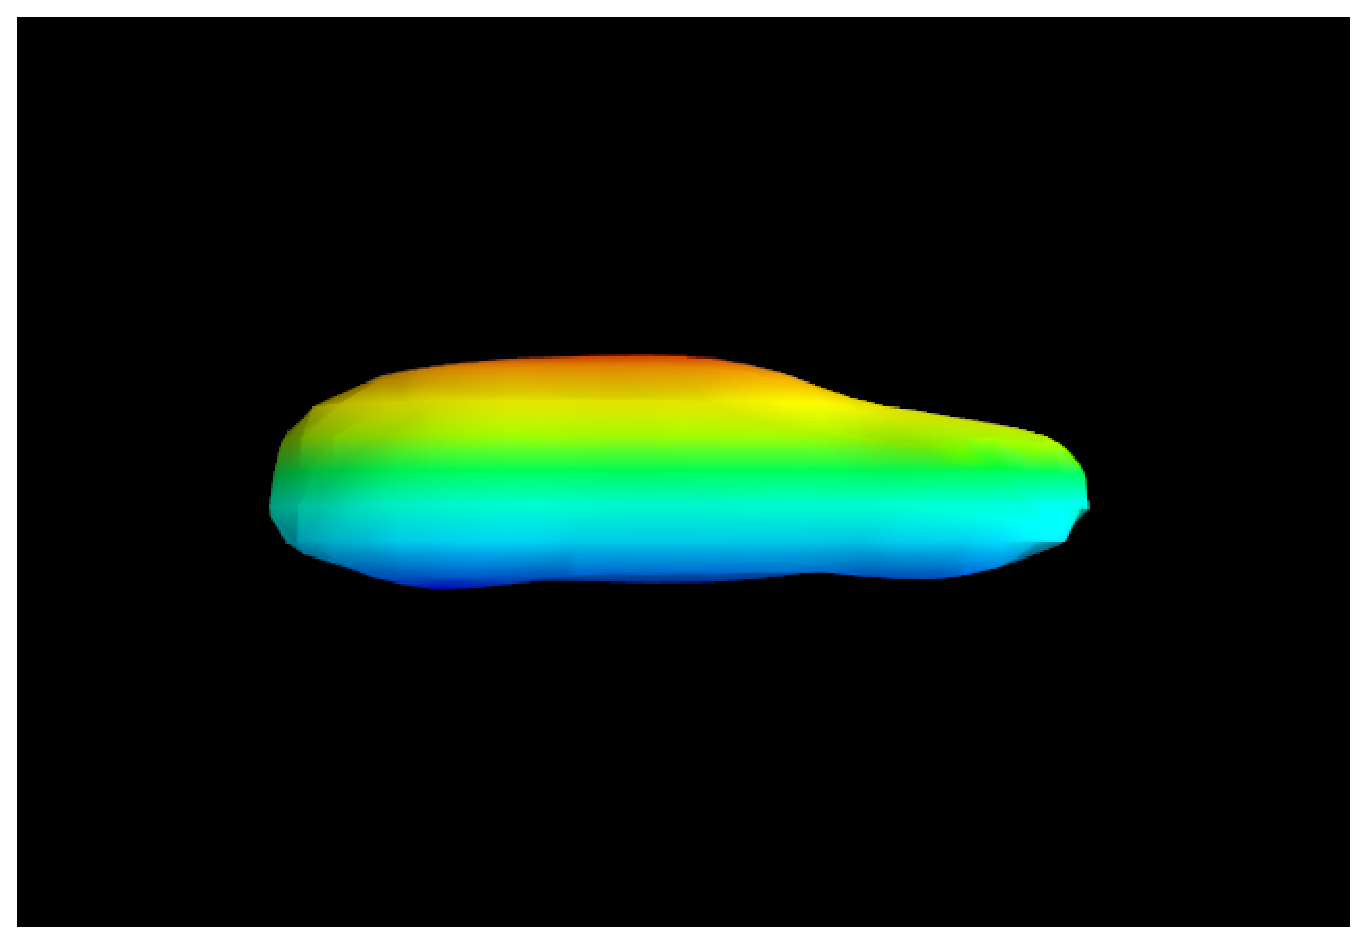
\includegraphics[width=.4\linewidth]{figures/spp/differing_harmonics/1_side.eps}\\
    (a) & (b) \\
    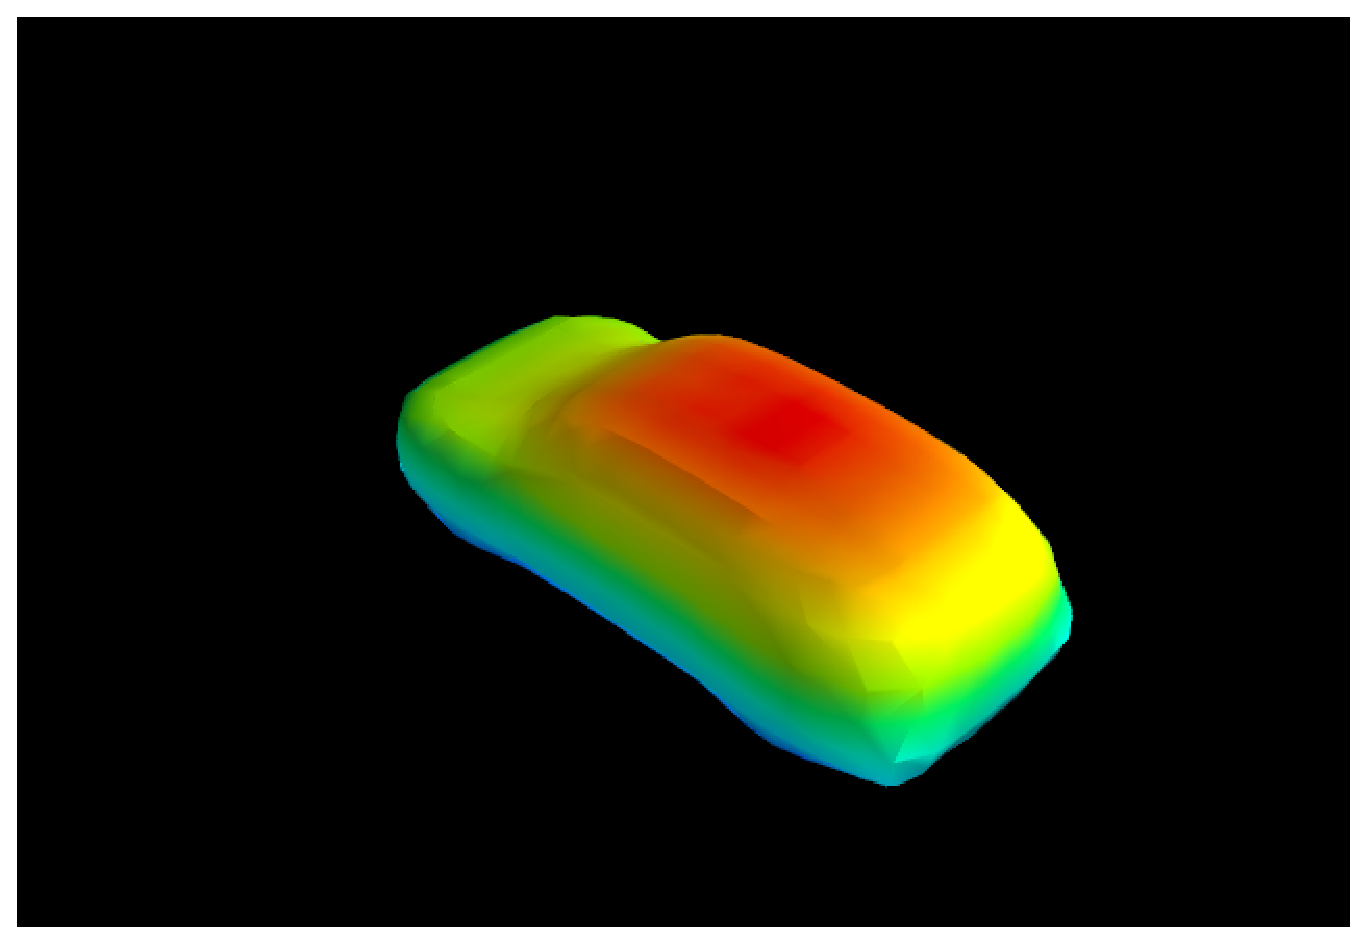
\includegraphics[width=.4\linewidth]{figures/spp/differing_harmonics/3.eps}&
		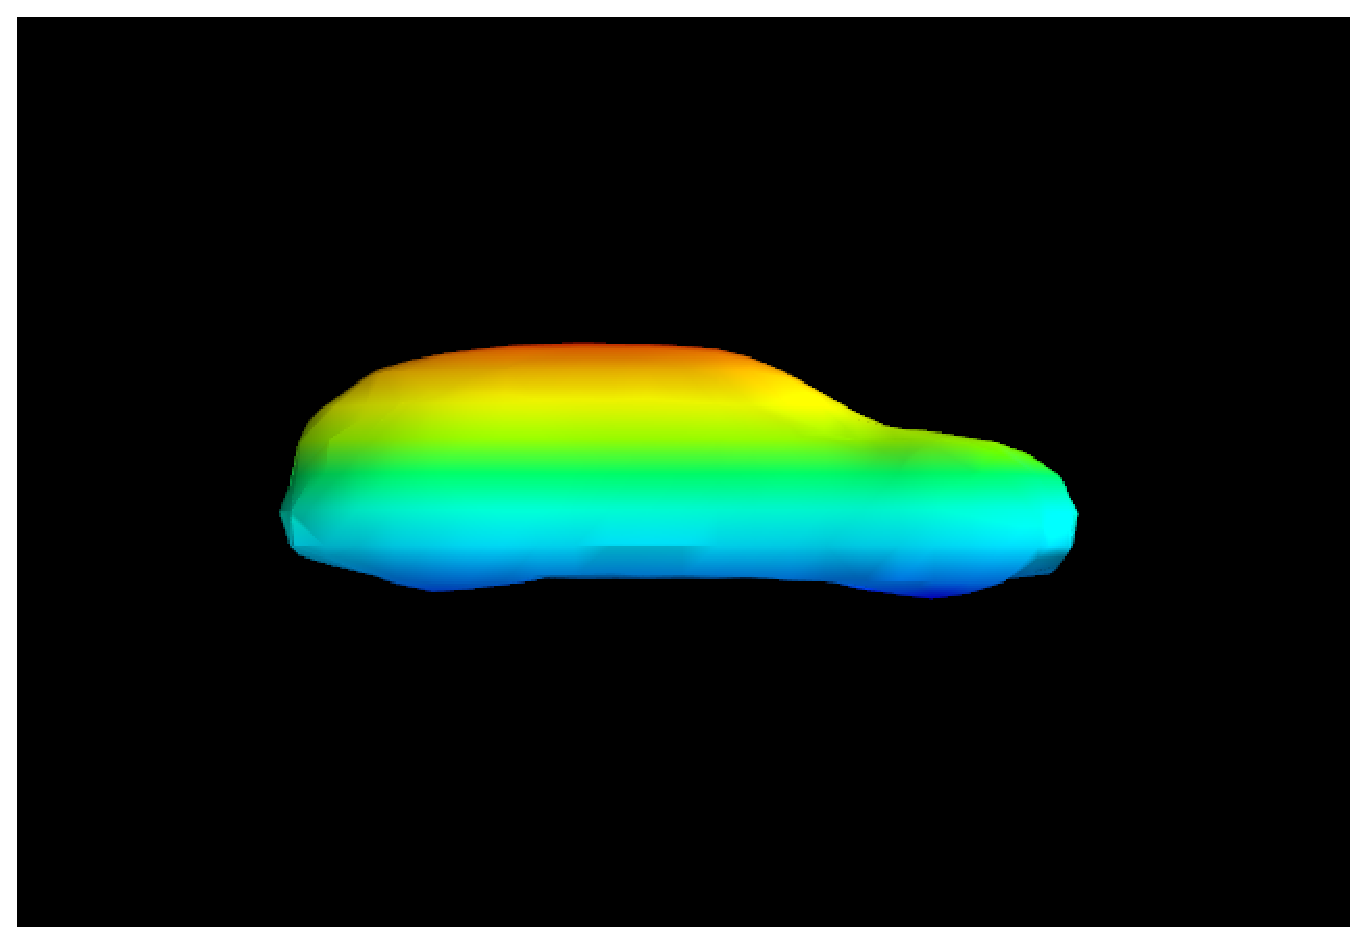
\includegraphics[width=.4\linewidth]{figures/spp/differing_harmonics/3_side.eps}\\
    (c) & (d) \\
    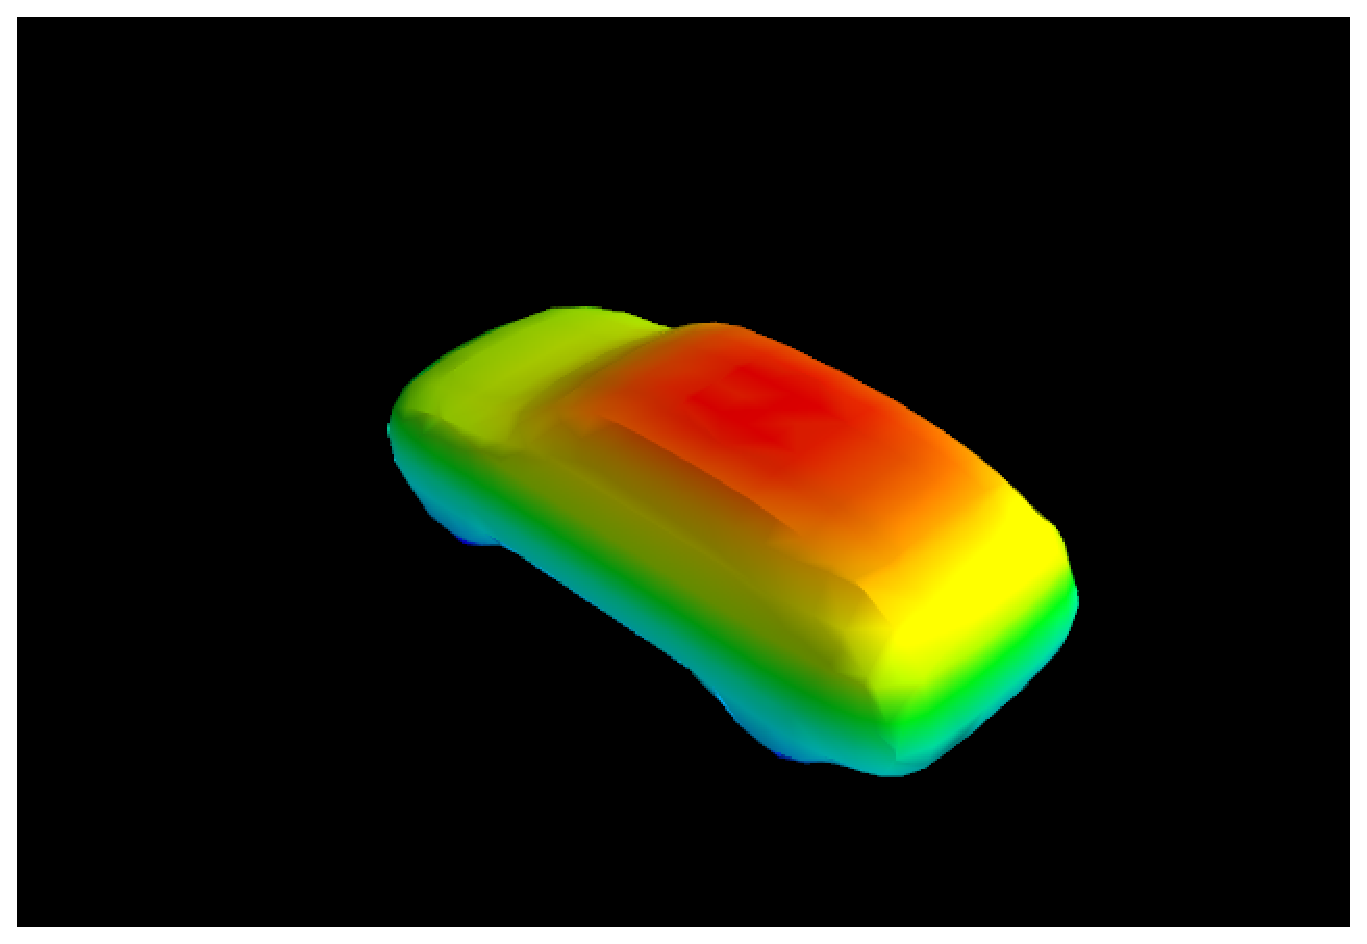
\includegraphics[width=.4\linewidth]{figures/spp/differing_harmonics/all.eps}&
		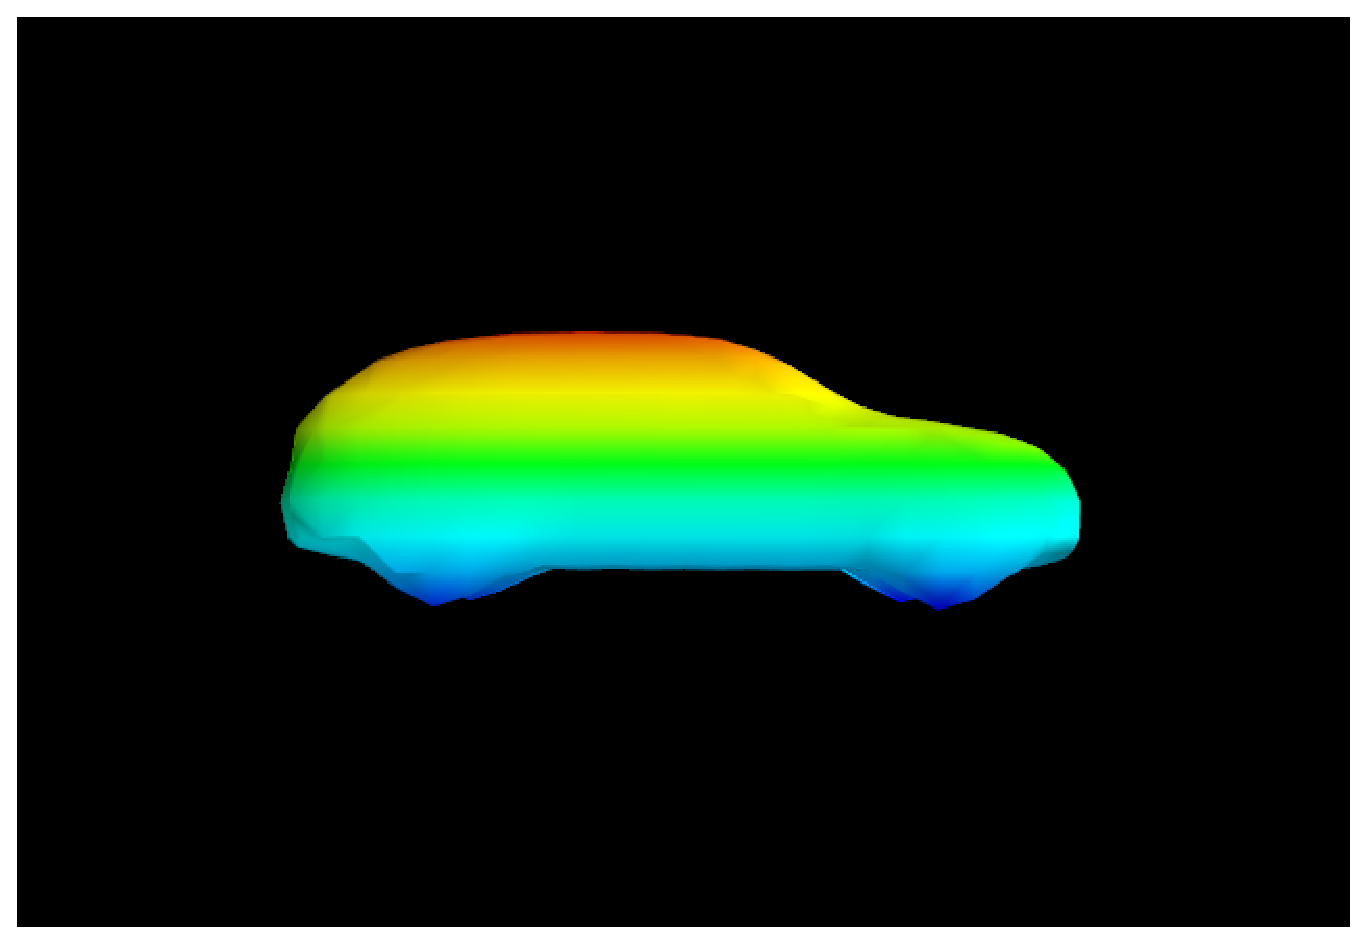
\includegraphics[width=.4\linewidth]{figures/spp/differing_harmonics/all_side.eps}\\
    (e) & (f)
  \end{tabular}
  \caption[SDF's generated with differing DCT harmonics.]
  {
    \begin{tabular}[t]{@{}l@{}}
      The effect of varying the number of DCT harmonics on the resultant\\ 3D shape is shown for:\\
      (a, b) One DCT harmonic.\\
      (c, d) Three DCT harmonics.\\
      (e, f) All DCT harmonics.\\
    \end{tabular}
  }
~\label{figure:spp_sdf_diff_harmonics}
\end{figure}

\subsection{Signed Distance Function Gradient}
~\label{subsec:spp_sdf_grad}
The SDF \( \bm{\Phi} \), generated by the IDCT given in Equation~\ref{eqn:spp_idct}, must be 
differentiable with respect to the posterior mean \( \bm{f}^{\star} \) for backpropagation 
training of the model. The gradient of the SDF \( \bm{\Phi} \) outlined in 
Equation~\ref{eqn:spp_idct} is derived as follows in Equation~\ref{eqn:spp_idct_grad}. 
For notational clarity, the DCT coefficients are defined as follows in Equation
~\ref{eqn:spp_dct_coeff}
\begin{equation}
  \label{eqn:spp_dct_coeff}
  \zeta(x, y, z) = 
  \cos \Big[ \frac{\pi \big( x^{2} + \frac{x}{2} \big)}{N} \Big]
  \cos \Big[ \frac{\pi \big( y^{2} + \frac{y}{2} \big)}{N} \Big]
  \cos \Big[ \frac{\pi \big( z^{2} + \frac{z}{2} \big)}{N} \Big]
\end{equation}
\begin{align}
  \label{eqn:spp_idct_grad}
  % Line 1.
  \frac{\partial \bm{\Phi}}{\partial \bm{f}_{x, y, z}^{\star}} ={}&
  \frac{\partial}{\partial \bm{f}_{x, y, z}^{\star}}
  \sum_{x=0}^{N-1} \sum_{y=0}^{N-1} \sum_{z=0}^{N-1} 
  \bm{f}^{\star}_{x, y, z} \zeta(x, y, z)\\
  % Line 2.
  ={}& \sum_{x=0}^{N-1} \sum_{y=0}^{N-1} \sum_{z=0}^{N-1} 
  \frac{\partial}{\partial \bm{f}_{x, y, z}^{\star}} \bm{f}^{\star}_{x, y, z}
  \zeta(x, y, z)\\
  % Line 3.
  ={}& \sum_{x=0}^{N-1} \sum_{y=0}^{N-1} \sum_{z=0}^{N-1} \Bigg[
    \Bigg[ 
      \frac{\partial}{\partial \bm{f}_{x, y, z}^{\star}} \bm{f}^{\star}_{x, y, z} 
    \Bigg] \zeta(x, y, z)
    + \bm{f}_{x, y, z}^{\star} \frac{\partial \zeta}{\partial \bm{f}_{x, y, z}^{\star}}
  \Bigg]\\
  % Line 4.
  ={}& \sum_{x=0}^{N-1} \sum_{y=0}^{N-1} \sum_{z=0}^{N-1}
  \nabla \bm{f}_{x, y, z}^{\star} \zeta(x, y, z)\\
  % Line 5.
  ={}& \sum_{x=0}^{N-1} \sum_{y=0}^{N-1} \sum_{z=0}^{N-1} 
  \nabla \bm{f}^{\star}_{x, y, z}
  \cos \Big[ \frac{\pi \big( x^{2} + \frac{x}{2} \big)}{N} \Big]
  \cos \Big[ \frac{\pi \big( y^{2} + \frac{y}{2} \big)}{N} \Big]
  \cos \Big[ \frac{\pi \big( z^{2} + \frac{z}{2} \big)}{N} \Big]
\end{align}

From Equation~\ref{eqn:spp_idct_grad} it is evident that the partial derivative 
\( \frac{\partial \bm{\Phi}}{\partial \bm{f}_{x, y, z}^{\star}} \) is trivial 
to compute, as the derivative of the IDCT is simply the IDCT of the derivative. 
Furthermore, the gradient of the posterior mean is similarly trivial to compute, as shown 
in Equation~\ref{eqn:spp_pos_mean_grad}.

\section{Pose Estimation}
~\label{sec:spp_pose_estim}
The parameters of the \( \mathbb{SE}(3) \) pose applied to the predicted shape are obtained 
from a fully connected component of the model, as outlined in Figure~\ref{figure:spp_pipeline}, as with the 
latent pose point of Section~\ref{subsec:sdf_extraction}.

The three rotational parameters \( \alpha \), \( \beta \) and \( \gamma \) are predicted by 
the pose network component of the model on the interval \( [-\pi, \pi) \). The translation parameters 
however do not have their output range restricted.

\section{Rendering}
~\label{sec:spp_rendering}
The dynamic SLAM and object reconstruction works of Chapters~\ref{chap:moseg} and~\ref{chap:probobj}, 
both rely on ray-casting to obtain a rendering of a surface embedded within an implicit volume, under 
some estimated pose. The approach taken in this chapter is very similar. 

Ray-casting is first and foremost used in the model outlined in Section~\ref{sec:spp_algorithm} for 
visualisation purposes, to render the estimated shape under the estimated pose for an instantaneous scene 
view. In Chapters~\ref{chap:moseg} and~\ref{chap:probobj}, the output rendering is also used for frame-wise 
evaluation and optimisation of the pose energy function. However, as the approach outlined in this chapter 
does not assume temporal consistency, the requirements for optimisation differ.

As the model outlined in Section~\ref{sec:spp_algorithm} relies on the backpropagation of gradients for it's 
training, the rendering module must be differentiable for the backward pass. As such, this section outlines a 
simple formulation of differentiable ray-casting, inspired by the work of \textit{Prisacariu et al}
~\cite{Prisacariu2011}. In addition to generating a shaded rendering, the proposed approach generates a 
probabilistic map. For a review of the generic ray-casting algorithm, refer to Section~\ref{subsec:moseg_static_rendering}.

By accumulating log probabilities of voxels visited on traversal of the ray, a differentiable representation 
of the process can be obtained. However, this relies on the use of a differentiable PDF\@. As with the approach 
to object reconstruction outlined in Chapter~\ref{chap:probobj}, the desired behaviour is that the distribution 
shall encode the probability of a voxel being very close to the isosurface embedded within the volume. As such, 
the log-sigmoid of Equation~\ref{eqn:probobj_surface_prior_cdf} is used. Thus, for a pixel location \( [x, y] \), 
the output probabilistic value is as follows in Equation~\ref{eqn:spp_diff_raycast}.
\begin{equation}
~\label{eqn:spp_diff_raycast}
\mathcal{R}(x, y) = \sum_{v \in \mathcal{V}} \ln P(v)
\end{equation}

In Equation~\ref{eqn:spp_diff_raycast}, \( \mathcal{V} \) is the set of voxels in the SDF \( \bm{\Phi} \) that 
intersect the ray from the given pixel in the image frame. The gradient of the \( \ln P(v) \) term in 
Equation~\ref{eqn:spp_diff_raycast} if the form given in Equation~\ref{eqn:probobj_log_post_rot_grad}.

\section{Multiple Task Loss}
~\label{sec:spp_loss}
The architecture outlined in Section~\ref{subsec:spp_network_architecture} contains multiple branches 
following the RoI extraction, each with a different task and associated loss function. As the approach outlined 
in this work is based on the \textit{Faster R-CNN}~\cite{Ren2015RCNN} architecture, the overall network loss 
is an aggregate of the individual task oriented losses, as outlined in Section~\ref{subsub:spp_neural_rpn}. 
As such, the overall network loss may be defined as follows in Equation~\ref{eqn:spp_overall_loss}.

\begin{equation}
  ~\label{eqn:spp_overall_loss}
  \mathcal{L} = 
  \mathcal{L}_{cls}(\bm{z}_{cls}, \bm{y}_{cls}) + 
  \mathcal{L}_{bb}(\bm{z}_{bb}, \bm{y}_{bb}) + 
  \mathcal{L}_{p}(\bm{z}_{p}, \bm{y}_{p}) + 
  \mathcal{L}_{s}(\bm{z}_{s}, \bm{y}_{s})
\end{equation}

In Equation~\ref{eqn:spp_overall_loss}, the four loss terms measure the models performance on 
classification, bounding box regression, pose regression and shape regression for predictions \( \bm{z} \) \
and targets \( \bm{y} \).

Note that the \( \mathcal{L}_{s} \) is a proxy loss over shape, which measures the similarity between 
the rendering of the predicted 3D shape under the predicted pose.

\subsection{Pose Loss}
~\label{sec:spp_pose_loss}
As the approach in this works assumes a known ground truth pose, a simple \( L_{2} \) loss over the 
network predicted pose parameters and the ground truth is sufficient. As outlined in Section~\ref{subsub:spp_neural_pose}, 
only the \( z \) component of the translation vector must be regressed by the network as the \( x \) and 
\( y \) components may be recovered from the predicted bounding box coordinates.

As such, the pose loss term is given in Equation~\ref{eqn:spp_pose_loss}, for rotational parameter vector 
\( \bm{z}_{\rho} \) and depth parameter \( z \).

\begin{equation}
  ~\label{eqn:spp_pose_loss}
  \mathcal{L}_{p} = \sum_{n=1}^{N} \Big[ \bm{y}_{\rho} - \bm{z}_{\rho} \Big]^{2} +
  \sum_{n=1}^{N} \Big[ \bm{y}_{z} - \bm{z}_{z} \Big]^{2}
\end{equation}

\section{Gradients for Training With Backpropagation}
~\label{sec:spp_backprop}
With the gradients of the model components derived, the gradient update to the neural network component 
may be given. As the proposed model is optimised using the backpropagation algorithm, 
the gradient update for layer \( n - m \) is computed by applying the chain rule to layer \( n \), 
successively working backwards to layer \( n - m \). As such, the gradient for the non CNN components 
with respect to the CNN output for pose \( \mathcal{O}_{p} \), is given as follows in Equation
~\ref{eqn:spp_grad_chain_pose}.
\begin{equation}
  \label{eqn:spp_grad_chain_pose}
  \frac{\partial \mathcal{L}}{\partial \mathcal{O}_{p}} = 
    \frac{\partial \mathcal{L}}{\partial \mathcal{R}}
    \frac{\partial \mathcal{R}}{\partial \bm{T}}
    \frac{\partial \bm{T}}{\partial \mathcal{O}_{p}}
\end{equation}

In Equation~\ref{eqn:spp_grad_chain_pose}, \( \mathcal{L} \) is the loss given in Equation~\ref{eqn:spp_overall_loss}
of Section~\ref{sec:spp_loss}, \( \mathcal{R} \) is the rendering of the predicted shape \( \bm{\Phi} \) under the 
predicted pose \( \bm{T} \) outlined in Section~\ref{sec:spp_rendering}. \( \bm{T} \) is the 
\( \mathbb{SE}(3) \) pose outlined in Section~\ref{sec:spp_pose_estim}. The gradient with respect 
to the latent shape point generated by CNN output \( \mathcal{O}_{l} \) may also be found in the same 
manner and is given in Equation~\ref{eqn:spp_grad_chain_latent}.
\begin{equation}
  \label{eqn:spp_grad_chain_latent}
  \frac{\partial \mathcal{L}}{\partial \mathcal{O}_{l}} = 
    \frac{\partial \mathcal{L}}{\partial \mathcal{R}}
    \frac{\partial \mathcal{R}}{\partial \mathcal{\bm{\Phi}}}
    \frac{\partial \bm{\Phi}}{\partial \bm{f}^{\star}}
    \frac{\partial \bm{f}^{\star}}{\partial \mathcal{O}_{l}}
\end{equation}

In Equation~\ref{eqn:spp_grad_chain_latent}, \( \mathcal{L} \) and \( \mathcal{R} \) 
are as in Equation~\ref{eqn:spp_grad_chain_pose}. \( \Phi \) is the SDF given by the IDCT, 
as given in Equation~\ref{eqn:spp_idct} of Section~\ref{subsec:sdf_extraction}. 
\( \bm{f}^{\star} \) is the posterior mean of the GPLVM, given by Equation
~\ref{eqn:spp_gp_posterior_draw}.

\section{Qualitative Results}
~\label{sec:spp_qualitative}
This section shall provide a qualitative evaluation of the approach outlined in this chapter, both with respect to shape 
and combined shape and pose. For the experiments in this section and Section~\ref{sec:spp_quantitative} two data sources were 
used. For the task of pose prediction, the \textit{VKITTI} dataset was chosen for it's accurate ground truth and relative 
\textit{real world} nature (photorealistic renderings of real world scenes). For the shape embedding and prediction component, 
the GPLVM model outlined in Section~\ref{sec:spp_gplvm} was trained on a collection of 3D shapes obtained from the online 
\textit{ShapeNet} collection of 3D CAD models\footnotemark. 
~\footnotetext{ShapeNet: https://www.shapenet.org/}

For the training of the generative model, 70 CAD models of cars were obtained from \textit{ShapeNet}, chosen to cover a variety 
of common geometries for the class. The obtained CAD models were then manually processed to remove inner geometry, voxelised into 
binary occupancy volumes and finally converted to SDF's by the computation of the Eucledian Distance Transform to the binarised 
contour. 

When training the latent shape point network, outlined in Section~\ref{subsub:spp_neural_latent}, a combination of the \textit{VKITTI} 
dataset and the shape drawn from the generative model of Section~\ref{sec:spp_gplvm} (derived from the \textit{ShapeNet} CAD models) 
is used. As outlined, the \textit{VKITTI} dataset contains both ground truth 6DoF pose and ground truth semantic segmentation masks. As 
outlined in Section~\ref{sec:spp_introduction}, the loss of Section~\ref{TODO} is minimised over the rendering of the shape drawn 
from the GP under the predicted pose, with respect to the ground truth mask. The 3D CAD models were also reoriented to align with the 
\textit{VKITTI} coordinate system of \( y \) pointing downwards, \( x \) pointing to the right and \( z \) directly forwards.

\subsection{Gaussian Process Latent Shape Embedding}
~\label{subsec:spp_qualitative_shape}
The GPLVM based embedding of 3D shape outlined in Section~\ref{sec:spp_gplvm} was trained on a small but varied dataset of 3D CAD 
models. Qualitatively, the trained model appears capable of representing common geometries of the class of interest in this work. 
Given in Figure~\ref{figure:spp_qualitative_shapes} are examples of shapes drawn from the shape distribution at uniformly sampled 
latent space points.

\begin{figure}[!htbp]
  \centering
  \begin{tabular}{cc}
    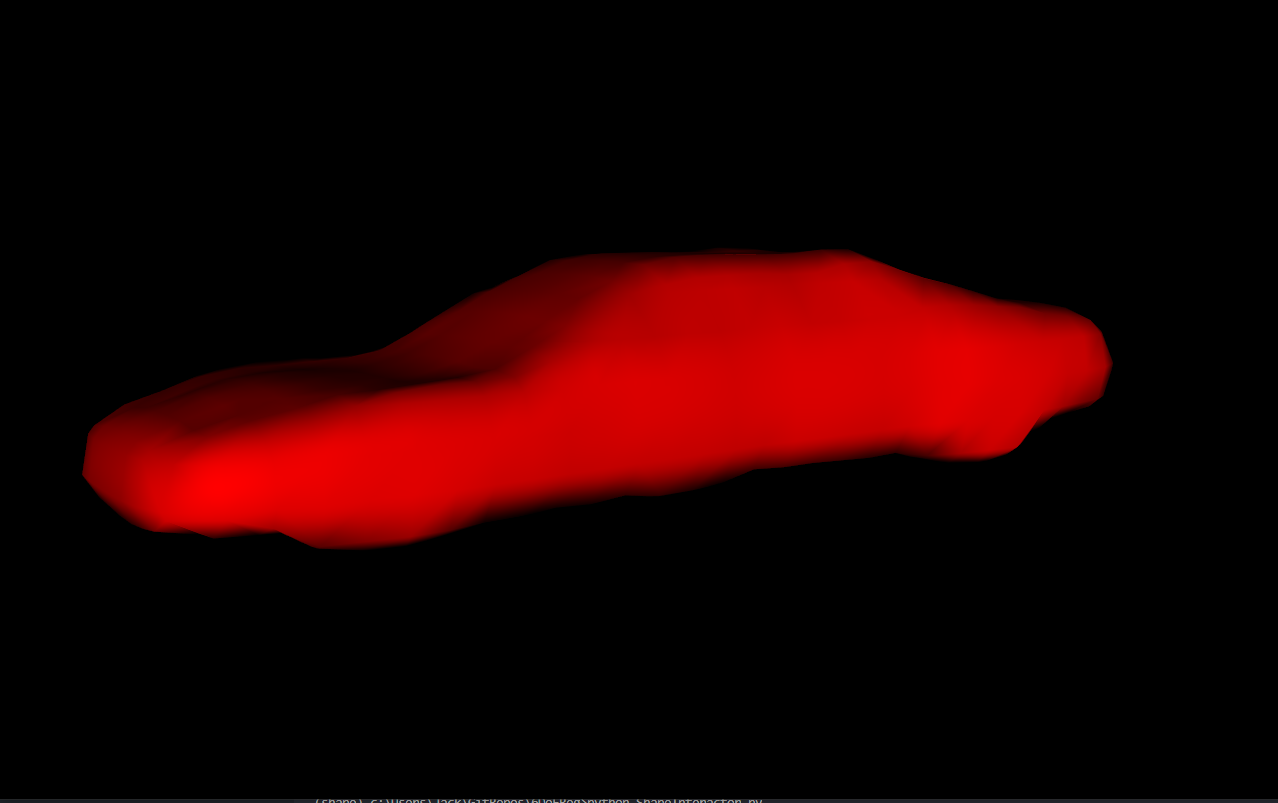
\includegraphics[width=.4\linewidth]{figures/spp/gp_draws/0.png}&
		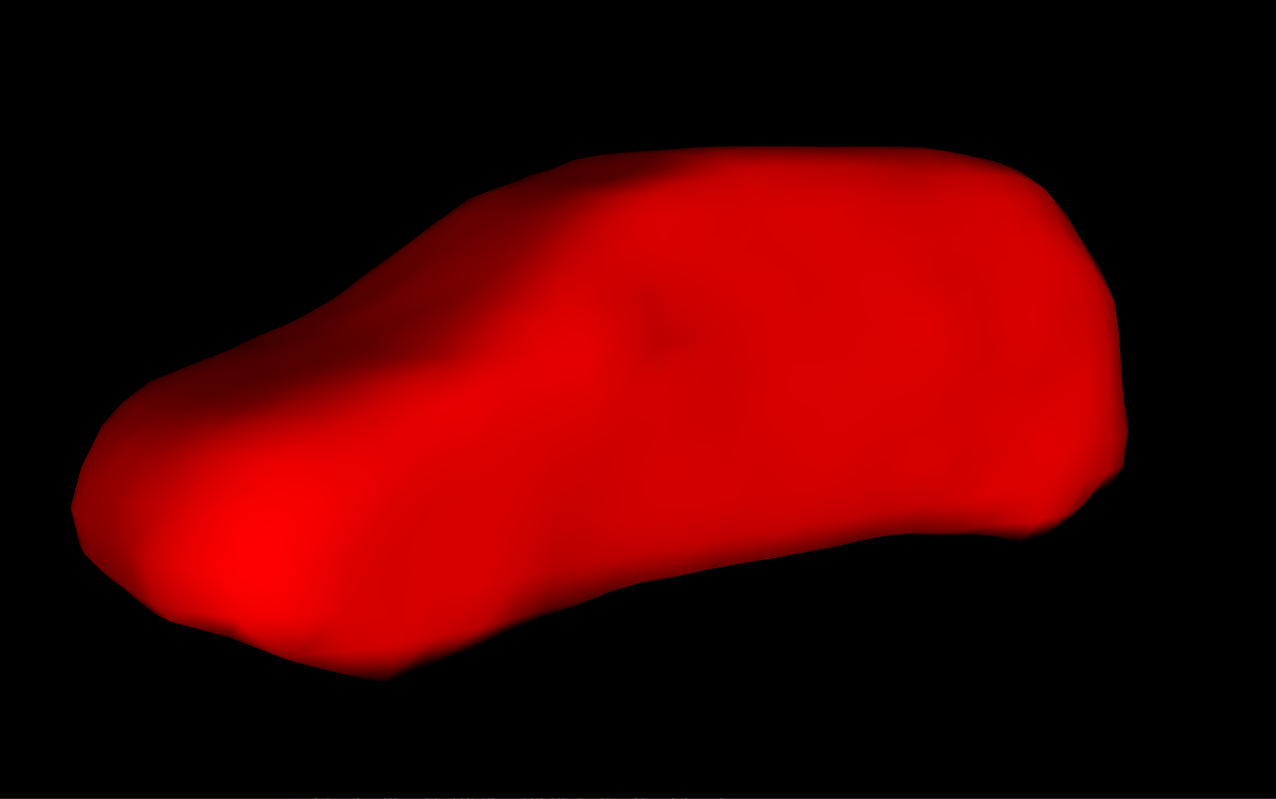
\includegraphics[width=.4\linewidth]{figures/spp/gp_draws/1.png}\\
    (a) & (b) \\
    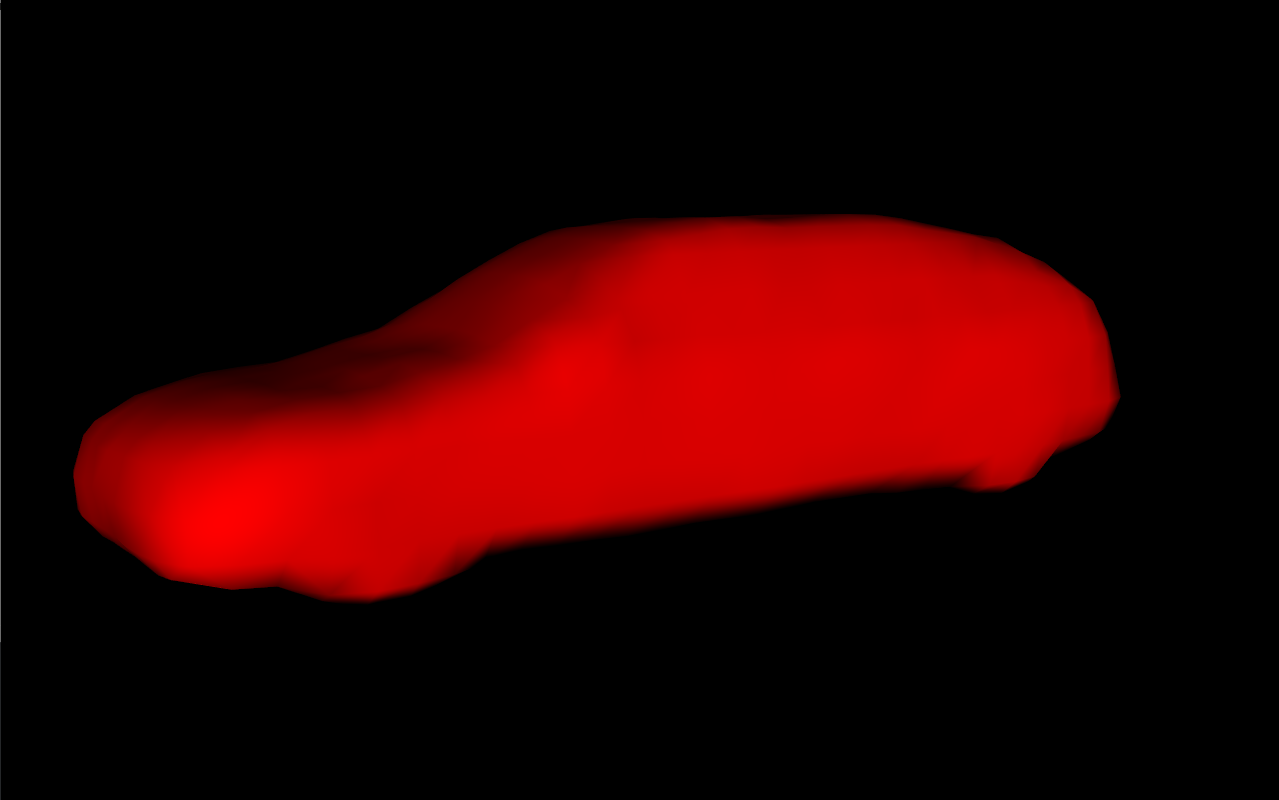
\includegraphics[width=.4\linewidth]{figures/spp/gp_draws/2.png}&
		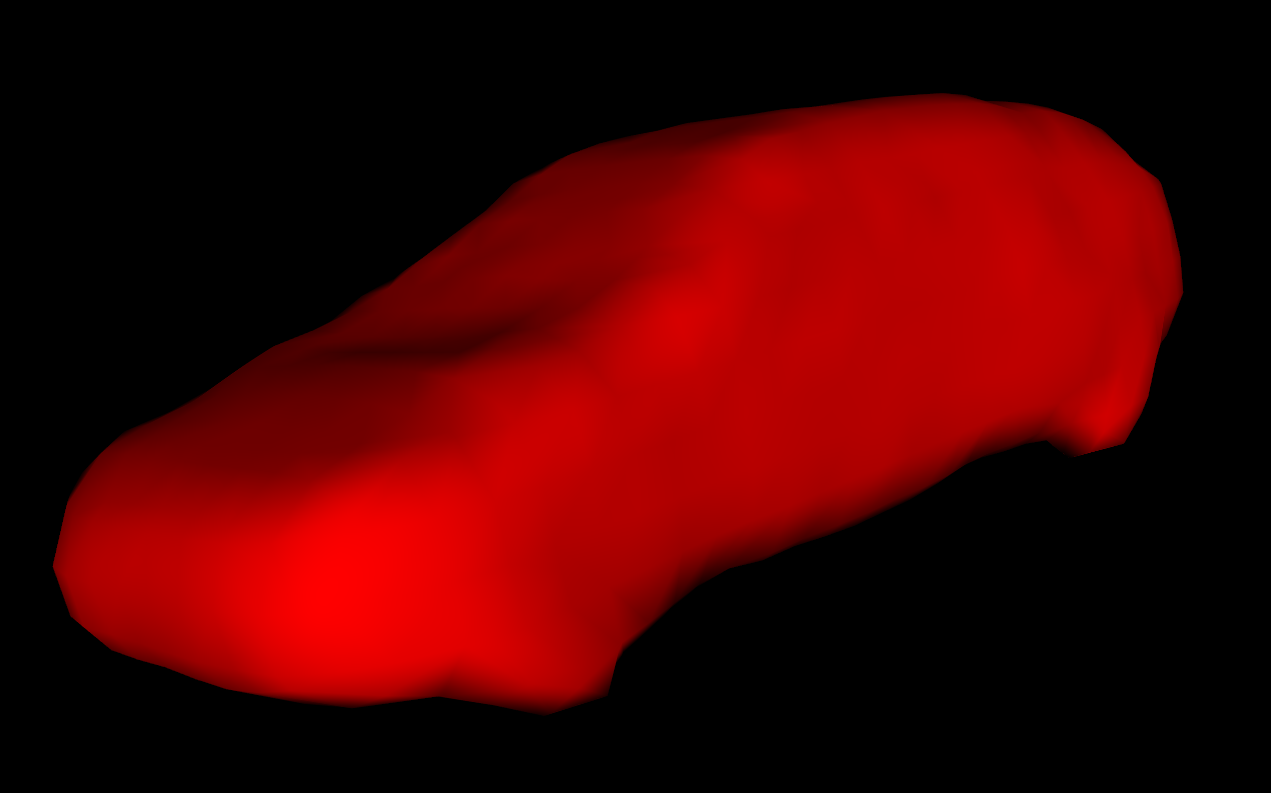
\includegraphics[width=.4\linewidth]{figures/spp/gp_draws/3.png}\\
    (c) & (d)
  \end{tabular}
  \caption[GP Shape Draws]
  {
    (a, b, c, d) IDCT extracted, random draws from the trained GP.
  }
~\label{figure:spp_qualitative_shapes}
\end{figure}

It can be seen in Figure~\ref{figure:spp_qualitative_shapes}, the trained shape model is capable of embdedding a variety of 
3D geometries relevant to the problem addressed in this work. Note that due to the probabilistic nature of the shape model, for 
a predicted shape (a posterior mean), there is additionally covariance information for each estimated posterior mean. The shapes 
given in Figure~\ref{figure:spp_qualitative_shapes} were drawn from a region of the latent space for which there is low covariance, 
thus higher probabilistic certainty. Figure~\ref{figure:spp_qualitative_shapes_bad} demonstrates shapes drawn from the shape distribution 
on regions of the latent space for which there is higher covariance and thus increased estimation uncertainty.

\begin{figure}[!htbp]
  \centering
  \begin{tabular}{cc}
    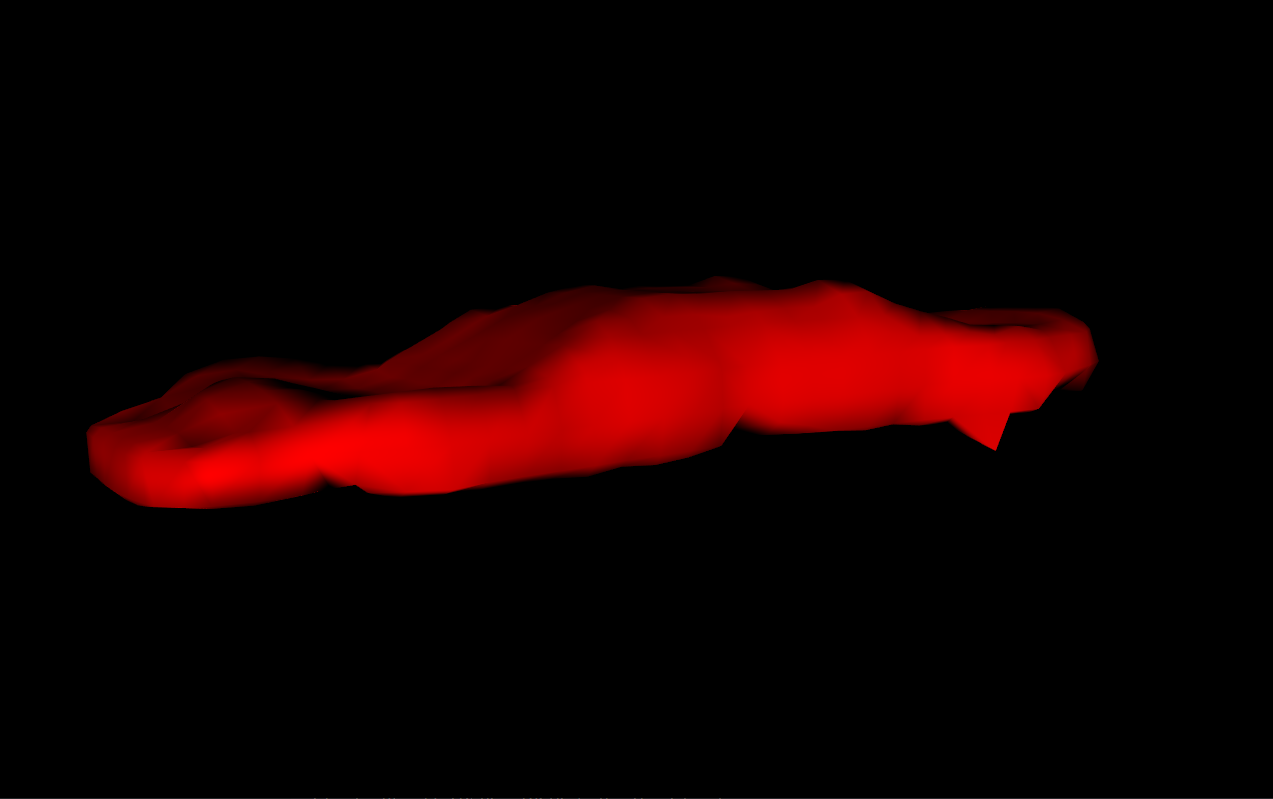
\includegraphics[width=.4\linewidth]{figures/spp/gp_draws/bad/0.png}&
		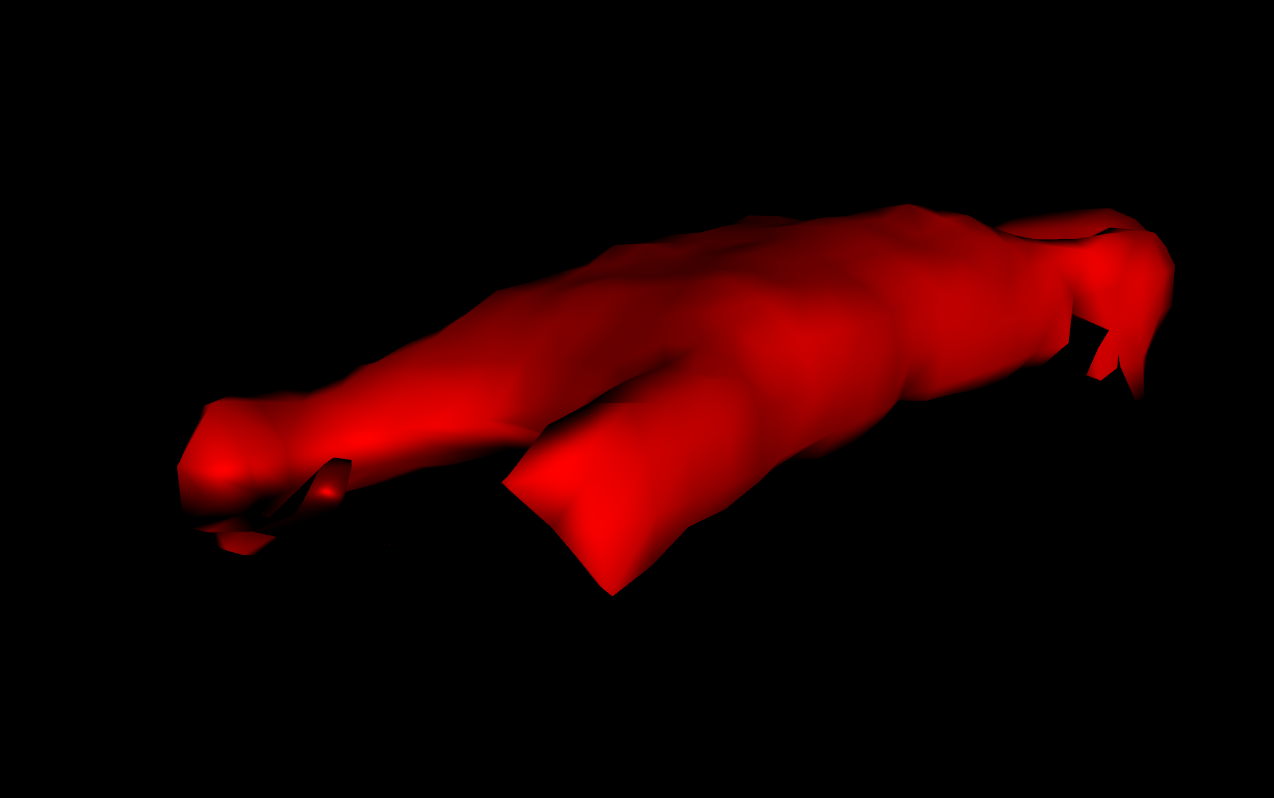
\includegraphics[width=.4\linewidth]{figures/spp/gp_draws/bad/1.png}\\
    (a) & (b)
  \end{tabular}
  \caption[Bad GP Shape Draws]
  {
    (a, b) IDCT extracted, random draws from the trained GP in regions of the latent 
    space that have high covariance.
  }
~\label{figure:spp_qualitative_shapes_bad}
\end{figure}

Given in Figure~\ref{figure:spp_qualitative_latent_cov} is a visual representation of the uncertainty 
in estimated shape with respect to the latent space point on which the GP is conditioned. The examples 
provided in Figures~\ref{figure:spp_qualitative_shapes} and~\ref{figure:spp_qualitative_shapes_bad} 
correspond to the low uncertainty (dark) and higher (light) uncertainty regions of 
Figure~\ref{figure:spp_qualitative_latent_cov}, respectively.

\begin{figure}[!htbp]
  \centering
  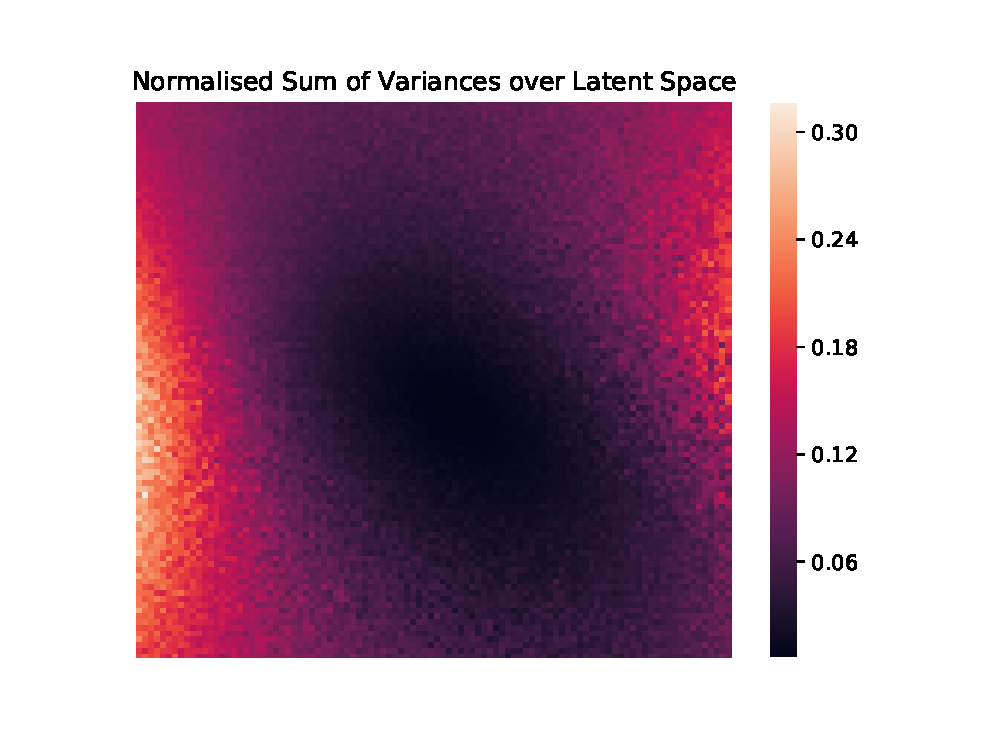
\includegraphics[width=\linewidth]{figures/spp/gp_latent_heatmap.eps}
  \caption[Latent Space Variance]{Normalised sum of the embedding variance for estimated shape on the latent 
  space, for regularly sampled latent points on the interval \( \left[-5, 5\right] \). Lower values indicate 
  lower estimation uncertainty.}
~\label{figure:spp_qualitative_latent_cov}
\end{figure}

\section{Quantitative Results}
~\label{sec:spp_quantitative}
Following the qualitative results presented in Section~\ref{sec:spp_qualitative}, this section 
provides a quantitative analysis of the performance of the model outlined in this work.

First, an overview of the models performance during training is provided, followed by quantitative 
results on the pose prediction performance of the model. Finally, a quantitative measure of the 
shape prediction performance of the model is provided. In the training sections that follow, the supervised 
and weakly supervised tasks have been trained and tested on a randomised \( 80:20 \) training and validation 
data split, respectively.

\subsection{Transfer Learning for Car Detection on VKITTI}
~\label{sec:spp_quantitative_transfer}
The training of the model has been performed in multiple stages. Firstly, the standard \textit{Faster R-CNN} 
is trained on the dataset outlined in Section~\ref{sec:spp_introduction} for the tasks of classification and 
bounding box regression. This stage of training may be thought of as a simple application of transfer learning 
for the specific problem domain outlined in this work; the backbone and RPN components of the network 
have been pretrained on the \textit{Microsoft Common Objects in Context (COCO)}~\cite{Lin2014COCO} dataset for 
the tasks of object classification and bounding box regression. Due to the specialisation of the detection 
requirements in this work, the RPN and feature extraction components must be retrained.

\begin{figure}[!htbp]
  \centering
  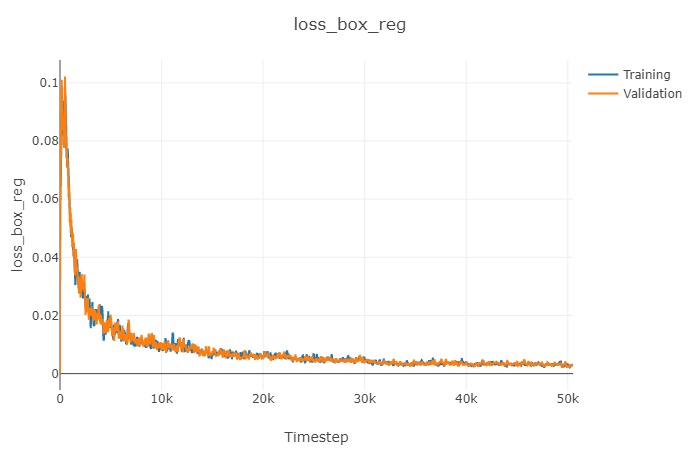
\includegraphics[width=.6\linewidth]{figures/spp/quant/rcnn_pretrain/bb.png}
  \caption[VKITTI Bounding Box Training]{Bounding box regression loss on the \textit{VKITTI} 
  dataset for the standard \textit{Faster R-CNN} network.}
~\label{figure:spp_pretrain_bb}
\end{figure}

Figure~\ref{figure:spp_pretrain_bb} depicts the short retraining of the RPN and finetuning of the feature extraction 
network of the model outlined in Section~\ref{sec:spp_algorithm}. It can be seen that in a relatively short training period, 
the \textit{Microsoft COCO} pretrained network rapidly becomes performant on the \textit{VKITTI} dataset used in this work, 
for the task of specific object detection. Additionally, similar behaviour may be observed in Figure~\ref{figure:spp_pretrain_cls} 
for the coupled task of object classification.

\begin{figure}[!htbp]
  \centering
  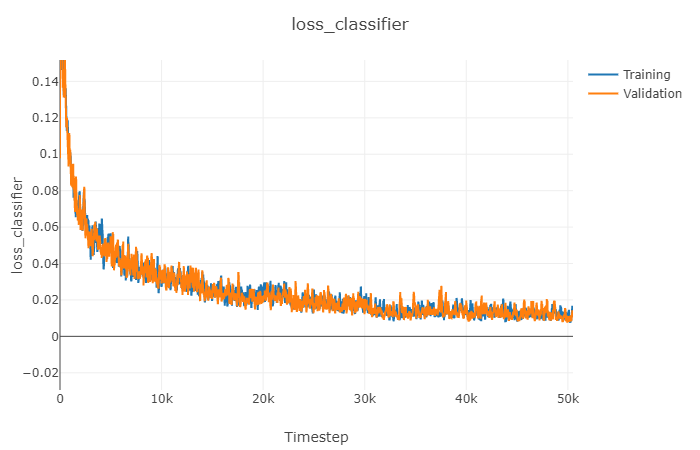
\includegraphics[width=.6\linewidth]{figures/spp/quant/rcnn_pretrain/cls.png}
  \caption[VKITTI Classification Training]{Classification loss on the \textit{VKITTI} 
  dataset for the standard \textit{Faster R-CNN} network.}
~\label{figure:spp_pretrain_cls}
\end{figure}

For the training procedures of Figures~\ref{figure:spp_pretrain_bb} and~\ref{figure:spp_pretrain_cls}, the Stochastic Gradient 
Descent (SGD) optimisation routine was used, with a learning rate of \( 0.001 \). The training session consisted of \(50,000\) 
batches, for which a batch consists of the class relevant ground truth detecions for a given frame.

\subsection{GPLVM Training}
~\label{sec:spp_quantitative_gp_train}
The training procedure of the GPLVM outlined in Section~\ref{sec:spp_gplvm} is an unsupervised routine and as such, 
no training/testing split of the 3D CAD model data introduced in Section~\ref{sec:spp_qualitative} is required. It 
can be seen in Figure~\ref{figure:spp_gplvm_train} that the GPLVM model requires very few iterations to converge to 
an optimal latent embedding. The model was trained by minimising the negative log-likelihood, as is standard in 
the GP literature~\cite{GPML}.

\begin{figure}[!htbp]
  \centering
  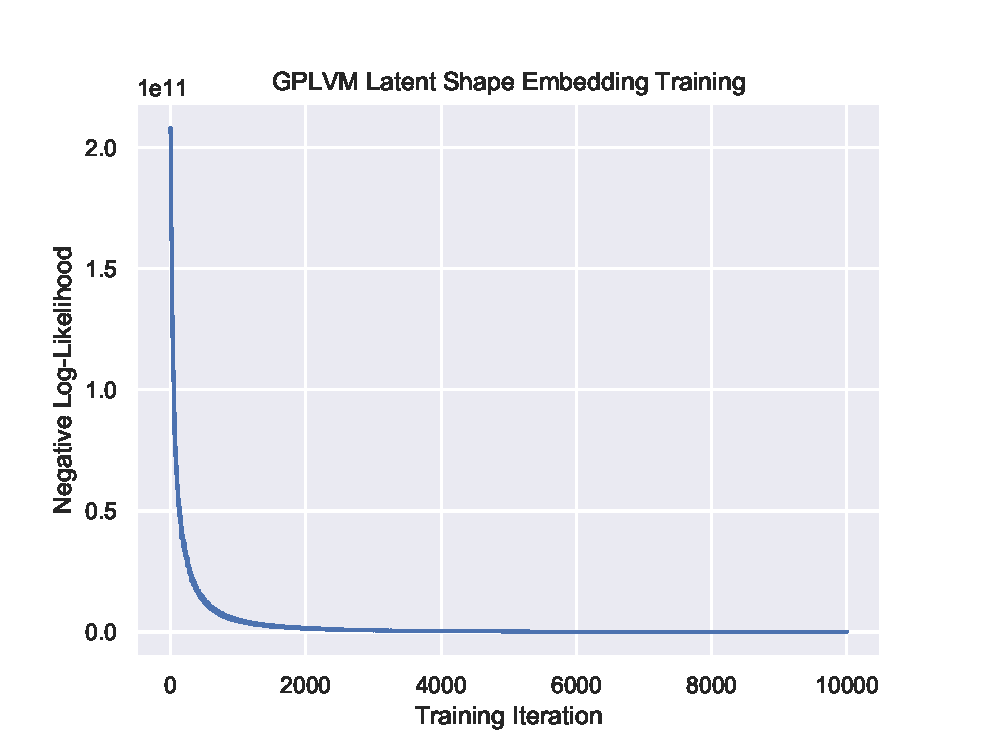
\includegraphics[width=.6\linewidth]{figures/spp/quant/gp_train.eps}
  \caption[VKITTI Classification Training]{Classification loss on the \textit{VKITTI} 
  dataset for the standard \textit{Faster R-CNN} network.}
~\label{figure:spp_gplvm_train}
\end{figure}

For the training procedure given in Figure~\ref{figure:spp_gplvm_train}, the Adam~\cite{Kingma2014} 
optimiser was used with a base learning rate of \( 0.01 \). The model was trained for 1500 epochs, 
though as can be seen in Figure~\ref{figure:spp_gplvm_train}, the model converges considerably 
prior to this epoch limit.

\subsection{Supervised Training of Pose}
~\label{sec:spp_quantitative_pose_train}

\subsection{Weakly Supervised Training of Latent Shape}
~\label{sec:spp_quantitative_latentshape_train}

\subsection{Pose Accuracy}
~\label{sec:spp_quantitative_pose_accuracy}

\subsection{Shape Accuracy}
~\label{sec:spp_quantitative_pose_accuracy}

\section{Summary}
~\label{sec:spp_discussion}
